
%%%%%%%%%%%%%%%%%%%%%%%%%%%%%%%%%%%%%%%%%
% Beamer Presentation
% LaTeX Template
% Version 1.0 (10/11/12)
%
% This template has been downloaded from:
% http://www.LaTeXTemplates.com
%
% License:
% CC BY-NC-SA 3.0 (http://creativecommons.org/licenses/by-nc-sa/3.0/)
%
%%%%%%%%%%%%%%%%%%%%%%%%%%%%%%%%%%%%%%%%%

%----------------------------------------------------------------------------------------
%	PACKAGES AND THEMES
%----------------------------------------------------------------------------------------

\documentclass{beamer}

\mode<presentation> {
	
	% The Beamer class comes with a number of default slide themes
	% which change the colors and layouts of slides. Below this is a list
	% of all the themes, uncomment each in turn to see what they look like.
	
	%\usetheme{default}
	%\usetheme{AnnArbor}
	%\usetheme{Antibes}
	%\usetheme{Bergen}
	%\usetheme{Berkeley}
	%\usetheme{Berlin}
	%\usetheme{Boadilla}
	%\usetheme{CambridgeUS}
	%\usetheme{Copenhagen}
	%\usetheme{Darmstadt}
	%\usetheme{Dresden}
	%\usetheme{Frankfurt}
	%\usetheme{Goettingen}
	%\usetheme{Hannover}
	%\usetheme{Ilmenau}
	%\usetheme{JuanLesPins}
	%\usetheme{Luebeck}
	%\usetheme{Madrid}
	%\usetheme{Malmoe}
	%\usetheme{Marburg}
	%\usetheme{Montpellier}
	%\usetheme{PaloAlto}
	%\usetheme{Pittsburgh}
	\usetheme{Rochester}
	%\usetheme{Singapore}
	%\usetheme{Szeged}
	%\usetheme{Warsaw}
	
	% As well as themes, the Beamer class has a number of color themes
	% for any slide theme. Uncomment each of these in turn to see how it
	% changes the colors of your current slide theme.
	
	%\usecolortheme{albatross}
	\usecolortheme{beaver}
	%\usecolortheme{beetle}
	%\usecolortheme{crane}
	%\usecolortheme{dolphin}
	%\usecolortheme{dove}
	%\usecolortheme{fly}
	%\usecolortheme{lily}
	%\usecolortheme{orchid}
	%\usecolortheme{rose}
	%\usecolortheme{seagull}
	%\usecolortheme{seahorse}
	%\usecolortheme{whale}
	%\usecolortheme{wolverine}
	
	%\setbeamertemplate{footline} % To remove the footer line in all slides uncomment this line
	%\setbeamertemplate{footline}[page number] % To replace the footer line in all slides with a simple slide count uncomment this line
	
	%\setbeamertemplate{navigation symbols}{} % To remove the navigation symbols from the bottom of all slides uncomment this line
}

\usepackage{graphicx} % Allows including images
\usepackage{booktabs} % Allows the use of \toprule, \midrule and \bottomrule in tables
%\usepackage{ctex}
\usepackage{multicol}

\usepackage{fontspec}
\setsansfont{Calibri}[
    Path=Font/,
    Scale=0.9,
    Extension = .ttf,
    UprightFont=*-Regular,
    BoldFont=*-Bold,
    ItalicFont=*-Italic,
    BoldItalicFont=*-BoldItalic
    ]
\usepackage{unicode-math}

% \setmathfont{Libertinus Math} % 使用默认的数学字体或你偏好的数学字体 Latin Modern Math

\usepackage{ragged2e}
\justifying\let\raggedright\justifying %两端对齐

%----------------------------------------------------------------------------------------
%	TITLE PAGE
%----------------------------------------------------------------------------------------

\title[Asset Pricing]{\textbf{Asset Pricing}} % The short title appears at the bottom of every slide, and the full title is only on the title page

\subtitle{2. Time-series Predictability (Literature)}

\author[Cheng Hang]{Cheng Hang} % Your name
\institute[DUFE] % Your institution as it will appear on the bottom of every slide, maybe shorthand to save space
{School of Fintech \\
	Dongbei University of Finance \& Economics \\ % Your institution for the title page
	\medskip
	\textbf{chenghangch@qq.com}% Your email address
}
\date{\today} % Date, can be changed to a custom date

\AtBeginSection[]
{
	\begin{frame}{Content}
		\begin{columns}[t]
			\begin{column}{0.5\textwidth}
				\tableofcontents[sections={1-2},sectionstyle=show/shaded,subsectionstyle=show/shaded/hide]
			\end{column}
			\begin{column}{0.5\textwidth}
				\tableofcontents[sections={3-4},sectionstyle=show/shaded,subsectionstyle=show/shaded/hide]
			\end{column}
		\end{columns}
		\addtocounter{framenumber}{-1}
	\end{frame}
}

%-----------------------------
%	Begin
%-----------------------------

\begin{document}
	
\begin{frame}
	\titlepage % Print the title page as the first slide
\end{frame}


\section{Valuation to Risk (Risk Return Trade Off)}
 %--- Slide 2: The Transition: Why move from Valuation to Risk? ---
\begin{frame}{Transition: From Valuation to Risk}
    \begin{itemize}
        \item \textbf{Previously:} We discussed predicting returns using valuation ratios like the Price-Dividend ratio ($pd$) and Consumption-Wealth ratio ($cay$).
        \item \textbf{The Economic Logic:} 
            \begin{itemize}
                \item Why do $pd$ and $cay$ forecast returns? 
                \item Because they track time-varying \textbf{discount rates}.
            \end{itemize}
        \item \textbf{The Core Question:} 
            \begin{itemize}
                \item What drives discount rates? \textbf{Risk.}
                \item Rational Asset Pricing suggests: High expected returns should compensate for high risk (Volatility).
            \end{itemize}
    \end{itemize}
    \vspace{0.5cm}
    \centering
    \textit{We now turn to the theoretical foundation of this relationship: The ICAPM.}
\end{frame}

%--- Slide 3: Theoretical Foundation (Merton's ICAPM) ---
\begin{frame}{The Intertemporal CAPM (Merton, 1973)}
    \begin{block}{The Core Theory}
        \href{https://doi.org/10.2307/1913811}{\textcolor{blue}{Merton (1973)}} provides the theoretical link between conditional mean returns and conditional variance:
        
    \end{block}

    \begin{equation}
        E_t [R_{t+1}] = \mu + \gamma \cdot \sigma_t^2 (R_{t+1})
    \end{equation}

    \begin{itemize}
        \item $E_t [R_{t+1}]$: Expected excess market return.
        \item $\sigma_t^2$: Conditional variance of the market (Risk).
        \item $\gamma$: The Coefficient of Relative Risk Aversion (RRA).
    \end{itemize}

    
    \textbf{Hypothesis:} Since investors are risk-averse ($\gamma > 0$), periods of high volatility ($\sigma_t^2$) should predict high future returns.
\end{frame}

%--- Slide 4: The Empirical Puzzle ---
\begin{frame}{The Risk-Return Puzzle}
    Despite the strong theory, empirical testing of $R_{t+1} = \alpha + \gamma \widehat{\sigma}_t^2 + \epsilon_{t+1}$ yields conflicting results.
    
    \begin{block}{The Problem}
        \begin{itemize}
            \item Many studies (e.g., \href{https://doi.org/10.1016/0304-405X(87)90045-6}{\textcolor{blue}{Campbell, 1987}}; \href{https://doi.org/10.1111/j.1540-6261.1993.tb05128.x}{\textcolor{blue}{Glosten, Jagannathan, and Runkle (1993)}} find an insignificant or even \textbf{negative} relationship between variance and returns.
        \end{itemize}
    \end{block}

    \textbf{Why does the model fail?}
\end{frame}

%--- Slide 5: Why Does the Model Fail? ---
\begin{frame}{Diagnosing the Failure: Three Hypotheses}
    \begin{enumerate}
        \item \textbf{Measurement Error in $\sigma_t^2$:}
            \begin{itemize}
                \item GARCH-based estimates are noisy proxies for true conditional variance.
                \item Errors-in-variables bias attenuates $\hat{\gamma}$ toward zero.
            \end{itemize}
        \item \textbf{Volatility Feedback Effect:}
            \begin{itemize}
                \item News about future volatility affects current prices.
                \item This creates a contemporaneous negative correlation that contaminates the predictive regression.
            \end{itemize}
        \item \textbf{Omitted State Variables:}
            \begin{itemize}
                \item The ICAPM includes hedging demand terms for state variables beyond variance.
                \item Omitting these induces bias in $\hat{\gamma}$.
            \end{itemize}
    \end{enumerate}
\end{frame}


%--- Slide: Realized Variance ---
\begin{frame}{Realized Variance: A Model-Free Measure}
    \begin{block}{Definition}
        The \textbf{Realized Variance} over day $t$ is the sum of squared daily returns:
        \begin{equation}\label{equ: RV}
            RV_t = \sum_{i=1}^{M} r_{t,i}^2
        \end{equation}
        where $r_{t,i}$ is the $i$-th daily return and $M$ is the number of intervals.
    \end{block}
    
    \textbf{Properties:}
    \begin{itemize}
        \item As $M \to \infty$, $RV_t \xrightarrow{p} \int_0^1 \sigma_s^2 ds$ (integrated variance).
        \item Model-free: No parametric assumptions on variance dynamics.
        \item More informative than squared daily returns.
    \end{itemize}
    
    \textbf{Challenge:} $RV_t$ measures \textit{realized} (past) variance, not \textit{expected} (future) variance.
\end{frame}

%--- Slide: Variance Estimation with Autocorrelation Adjustment ---
\begin{frame}{Autocorrelation-Adjusted Variance (\href{https://doi.org/10.1016/0304-405X(87)90026-2}{\textcolor{blue}{French, Schwert, Stambaugh, 1987}})}
    \textbf{Problem:} Equation \textcolor{red}{(\ref{equ: RV})} ignores autocovariance and is \textbf{inconsistent} when \\
    \begin{equation*}
        Cov(r_t, r_{t-1}) \neq 0
    \end{equation*}

    \begin{block}{Adjusted Estimator (FSS, 1987)}
        \begin{equation}
            \hat{\sigma}^2_{adj} = \sum_{t=1}^{N} r_t^2 + 2\sum_{t=2}^{N} r_t r_{t-1}
        \end{equation}
    \end{block}
    
    \begin{itemize}
        \item First term: Sum of squared daily returns (standard RV).
        \item Second term: Adjustment for first-order autocorrelation.
        \item Factor of 2 accounts for symmetric covariance structure.
    \end{itemize}
\end{frame}

%--- Slide: Derivation and Intuition ---
\begin{frame}{Derivation: Why the Adjustment Term?}
    \textbf{Setup:} Monthly return is the sum of $N$ daily returns: $R_{monthly} = \sum_{t=1}^{N} r_t$
    
    \begin{block}{Variance of Monthly Return}
        \begin{align}
            Var(R_{monthly}) &= Var\left(\sum_{t=1}^{N} r_t\right) \nonumber \\
            &= \sum_{t=1}^{N} Var(r_t) + 2\sum_{t=2}^{N} Cov(r_t, r_{t-1}) + \cdots
        \end{align}
    \end{block}
    \begin{itemize}
        \item If returns are i.i.d., all covariance terms vanish.
        \item If returns are positively autocorrelated ($\rho_1 > 0$), the naive estimator \textbf{underestimates} true variance.
        \item FSS (1987) include only the first-order term, \textbf{assuming higher-order autocorrelations are negligible}.
    \end{itemize}
\end{frame}

%--- Slide: General Form ---
\begin{frame}{Generalized Autocorrelation Adjustment}
    For higher-order autocorrelation, the general formula is:
    
    \begin{block}{Hansen-Hodrick / Newey-West Style Adjustment}
        \begin{equation}
            \hat{\sigma}^2_{adj} = \sum_{t=1}^{N} r_t^2 + 2\sum_{j=1}^{q} \sum_{t=j+1}^{N} r_t r_{t-j}
        \end{equation}
        where $q$ is the number of autocovariance lags included.
    \end{block}
    
    \textbf{FSS (1987) Choice:} $q = 1$ (first-order only)
    \begin{itemize}
        \item Empirically, first-order autocorrelation dominates in daily stock returns.
        \item Sources: nonsynchronous trading, bid-ask bounce, partial price adjustment.
        \item Higher-order terms add noise without substantial bias reduction.
    \end{itemize}
\end{frame}

%--- Slide 6: The Volatility Feedback Hypothesis ---
\begin{frame}{Volatility Feedback (\href{https://doi.org/10.1016/0304-405X(92)90037-X}{\textcolor{blue}{Campbell \& Hentschel, 1992}})}
    \begin{block}{The Mechanism}
        \begin{enumerate}
            \item Bad news arrives $\Rightarrow$ Expected future volatility rises.
            \item Higher volatility $\Rightarrow$ Higher required returns (ICAPM).
            \item Higher discount rates $\Rightarrow$ \textbf{Prices fall today}.
        \end{enumerate}
    \end{block}
    \textbf{Implication:} 
    \begin{itemize}
        \item A positive volatility shock is associated with a \textit{contemporaneous} negative return.
        \item This ``leverage effect'' (or volatility feedback) obscures the positive \textit{predictive} relationship.
    \end{itemize}
    \vspace{0.3cm}
    \centering
    \textit{The true risk-return tradeoff is masked by this endogenous price response.}
\end{frame}

\subsection{\href{https://doi.org/10.1111/j.1540-6261.2006.00877.x}{\textcolor{blue}{Guo and Whitelaw, 2006}}}

%--- Slide: Introduction to Guo and Whitelaw (2006) ---
\begin{frame}{Uncovering the Risk-Return Relation (\href{https://doi.org/10.1111/j.1540-6261.2006.00877.x}{\textcolor{blue}{Guo and Whitelaw, 2006}})}
    \textbf{The Puzzle:}
    \begin{itemize}
        \item Simple regressions of returns on conditional variance yield weak or negative estimates.
        \item This contradicts the ICAPM prediction that $\gamma > 0$.
    \end{itemize}
    
    \vspace{0.3cm}
    \textbf{Their Thesis:}
    \begin{itemize}
        \item The failure is due to \textbf{omitted variable bias}, not a failure of theory.
        \item The full ICAPM includes a \textbf{hedge component} that is correlated with variance.
        \item Omitting this component biases the estimate of the risk-return tradeoff.
    \end{itemize}
    
    \vspace{0.3cm}
    \centering
    \textit{``There is a risk-return relation, but you need to look in the right place.''}
\end{frame}

%--- Slide: Theoretical Framework ---
\begin{frame}{Theoretical Framework: The Complete ICAPM}
    \textbf{Merton's (1973) ICAPM:} Expected excess return has two components.
    
    \begin{block}{The Two-Factor ICAPM}
        \begin{equation}
            E_t[R_{m,t+1}] = \gamma_t \cdot \sigma_{m,t}^2 + \lambda_t \cdot \sigma_{mf,t}
        \end{equation}
    \end{block}
    
    \begin{itemize}
        \item \textbf{First term:} Compensation for bearing market risk.
            \begin{itemize}
                \item $\gamma_t$: Coefficient of relative risk aversion.
                \item $\sigma_{m,t}^2$: Conditional variance of market return.
            \end{itemize}
        \item \textbf{Second term:} Hedge demand component.
            \begin{itemize}
                \item $\lambda_t$: Price of hedge risk.
                \item $\sigma_{mf,t}$: Conditional covariance between market return and state variable $f$.
            \end{itemize}
    \end{itemize}
    
    \textbf{Key Point:} Most studies estimate only the first term, ignoring the hedge component.
\end{frame}

%--- Slide: The Omitted Variable Problem ---
\begin{frame}{The Omitted Variable Problem}
    \textbf{What happens when we omit the hedge component?}
    
    Consider the misspecified regression:
    \begin{equation}
        R_{t+1} = \alpha + \gamma \sigma_t^2 + \epsilon_{t+1}
    \end{equation}
    
    \begin{block}{Omitted Variable Bias Formula}
        \begin{equation}
            \text{plim } \hat{\gamma} = \gamma + \lambda \cdot \frac{Cov(\sigma_{m,t}^2, \sigma_{mf,t})}{Var(\sigma_{m,t}^2)}
        \end{equation}
    \end{block}
    
    \textbf{Guo and Whitelaw's Insight:}
    \begin{itemize}
        \item If $\lambda > 0$ (investors demand compensation for hedge risk).
        \item And $Cov(\sigma_{m,t}^2, \sigma_{mf,t}) < 0$ (variance and hedge component are negatively correlated).
        \item Then $\hat{\gamma}$ is \textbf{biased downward}, potentially becoming negative.
    \end{itemize}
\end{frame}

%--- Slide: Why Negative Covariance? ---
\begin{frame}{Why is $Cov(\sigma_{m,t}^2, \sigma_{mf,t}) < 0$?}
    \textbf{Economic Intuition:}
    
    \begin{enumerate}
        \item \textbf{Countercyclical Variance:}
            \begin{itemize}
                \item Market variance is high during recessions (bad times).
                \item High variance signals poor investment opportunities.
            \end{itemize}
        
        \item \textbf{Procyclical Investment Opportunities:}
            \begin{itemize}
                \item Expected returns (investment opportunities) are high in bad times.
                \item The hedge component captures changes in these opportunities.
            \end{itemize}
        
        \item \textbf{Negative Correlation:}
            \begin{itemize}
                \item When variance rises, investment opportunities deteriorate.
                \item The covariance between returns and changes in opportunities becomes negative.
                \item Hence $Cov(\sigma_{m,t}^2, \sigma_{mf,t}) < 0$.
            \end{itemize}
    \end{enumerate}
    
    \textbf{Result:} The hedge component ``absorbs'' part of the risk premium, making $\hat{\gamma}$ appear small or negative.
\end{frame}

%--- Slide: Empirical Strategy ---
\begin{frame}{Empirical Strategy}
    \textbf{Challenge:} The hedge component $\sigma_{mf,t}$ is unobservable.
    
    \begin{block}{Solution: Use $cay$ as a Proxy}
        \href{https://doi.org/10.1111/0022-1082.00347}{\textcolor{blue}{Lettau and Ludvigson (2001)}}'s consumption-wealth ratio:
        \begin{equation}
            cay_t = c_t - \hat{\omega} a_t - (1-\hat{\omega}) y_t
        \end{equation}
        where $c$ = consumption, $a$ = asset wealth, $y$ = labor income.
    \end{block}
    
    \textbf{Why $cay$?}
    \begin{itemize}
        \item $cay$ forecasts stock returns (captures time-varying expected returns).
        \item $cay$ tracks the state of investment opportunities.
        \item Changes in $cay$ proxy for innovations to investment opportunities.
    \end{itemize}
\end{frame}

%--- Slide: The Augmented Regression ---
\begin{frame}{The Augmented Regression}
    \textbf{Guo and Whitelaw estimate:}
    
    \begin{block}{Full Specification}
        \begin{equation}
            R_{t+1} = \alpha + \gamma \cdot \sigma_t^2 + \delta \cdot cay_t + \phi \cdot \sigma_t^2 \times cay_t + \epsilon_{t+1}
        \end{equation}
    \end{block}
    
    \textbf{Interpretation of Coefficients:}
    \begin{itemize}
        \item $\gamma$: Risk-return tradeoff (now controlling for hedge demand).
        \item $\delta$: Direct effect of investment opportunities on expected returns.
        \item $\phi$: Interaction effect (time-varying risk aversion).
    \end{itemize}
    
    \vspace{0.3cm}
    \textbf{Alternative Specification:}
    \begin{equation}
        R_{t+1} = \alpha + \gamma \cdot \sigma_t^2 + \beta \cdot \widehat{h}_t + \epsilon_{t+1}
    \end{equation}
    where $\widehat{h}_t$ is a constructed hedge component based on $cay$.
\end{frame}

%--- Slide: Main Empirical Findings ---
\begin{frame}{Main Empirical Findings}
    \textbf{Data:} U.S. stock market, 1952--2000 (quarterly frequency).
    
    \begin{block}{Key Results}
        \begin{table}[h]
            \centering
            \footnotesize
            \begin{tabular}{lcc}
                \hline
                \textbf{Specification} & $\hat{\gamma}$ & \textbf{t-statistic} \\
                \hline
                Simple: $R$ on $\sigma^2$ & $-1.34$ & $-0.52$ \\
                With $cay$: $R$ on $\sigma^2$, $cay$ & $4.87$ & $2.14$ \\
                Full: $R$ on $\sigma^2$, $cay$, $\sigma^2 \times cay$ & $5.23$ & $2.31$ \\
                With hedge component & $6.12$ & $2.45$ \\
                \hline
            \end{tabular}
        \end{table}
    \end{block}
    
    \textbf{Interpretation:}
    \begin{itemize}
        \item Simple regression: $\gamma$ is negative and insignificant.
        \item Controlling for $cay$: $\gamma$ becomes \textbf{positive and significant}.
        \item Implied RRA: $\gamma \approx 5$--$6$ (economically plausible).
    \end{itemize}
\end{frame}

%--- Slide: The Partial Correlation ---
\begin{frame}{Understanding the Partial Correlation}
    \textbf{Guo and Whitelaw's Key Insight:}
    
    \begin{itemize}
        \item The \textit{unconditional} correlation between $\sigma_t^2$ and $E_t[R_{t+1}]$ is weak.
        \item But the \textit{partial} correlation (controlling for $cay$) is strongly positive.
    \end{itemize}
    
    \begin{block}{Decomposition}
        \begin{align}
            Corr(\sigma_t^2, E_t[R_{t+1}]) &= \underbrace{Corr(\sigma_t^2, \gamma\sigma_t^2)}_{\text{Direct effect } (+)} \nonumber \\
            &+ \underbrace{Corr(\sigma_t^2, \lambda\sigma_{mf,t})}_{\text{Indirect effect } (-)}
        \end{align}
    \end{block}
    
    \textbf{The negative indirect effect offsets the positive direct effect.}
    
    \vspace{0.2cm}
    Only by controlling for the hedge component can we isolate the true risk-return tradeoff.
\end{frame}

%--- Slide: Time-Varying Risk Aversion ---
\begin{frame}{Time-Varying Risk Aversion}
    \textbf{Additional Finding:} The risk-return tradeoff varies over the business cycle.
    
    \begin{block}{Interaction Effect}
        \begin{equation}
            E_t[R_{t+1}] = \gamma_0 \cdot \sigma_t^2 + \gamma_1 \cdot \sigma_t^2 \times cay_t + \lambda \cdot cay_t
        \end{equation}
    \end{block}
    
    \textbf{Interpretation:}
    \begin{itemize}
        \item When $cay$ is high (good times), risk aversion is lower.
        \item When $cay$ is low (bad times), risk aversion is higher.
        \item The price of risk $\gamma_t = \gamma_0 + \gamma_1 \cdot cay_t$ is countercyclical.
    \end{itemize}
    
    \vspace{0.3cm}
    \textbf{Economic Implication:} Investors demand higher compensation for risk during recessions, consistent with habit formation and long-run risk models.
\end{frame}


\subsection{\href{https://doi.org/10.1093/rfs/hhp008}{\textcolor{blue}{Bollerslev, Tauchen, and Zhou, 2009}}}

%--- Slide: Why Decompose Variance? ---
\begin{frame}{Why Decompose Variance?}
    \textbf{The Fundamental Problem:}
    \begin{itemize}
        \item ICAPM predicts: $E_t[R_{t+1}] = \gamma \cdot E_t[\sigma_{t+1}^2]$
        \item But we observe $\sigma_t^2$ (realized), not $E_t[\sigma_{t+1}^2]$ (expected).
        \item Using realized variance conflates predictable and unpredictable components.
    \end{itemize}
    
    \vspace{0.3cm}
    \textbf{Key Insight:}
    \begin{itemize}
        \item Only the \textit{expected} component should command a risk premium.
        \item The \textit{unexpected} component creates contamination (volatility feedback).
        \item Proper identification requires separating these two components.
    \end{itemize}
    
    \vspace{0.3cm}
    \centering
    \textit{The solution: Decompose variance and identify what is actually priced.}
\end{frame}

%--- Slide: The Variance Decomposition ---
\begin{frame}{The Variance Decomposition}
    \textbf{Total variance at time $t+1$ can be decomposed:}
    
    \begin{block}{Decomposition}
        \begin{equation}
            \sigma_{t+1}^2 = \underbrace{E_t[\sigma_{t+1}^2]}_{\text{Expected Variance}} + \underbrace{(\sigma_{t+1}^2 - E_t[\sigma_{t+1}^2])}_{\text{Variance Innovation}}
        \end{equation}
    \end{block}
    
    \textbf{Component 1: Expected Variance $E_t[\sigma_{t+1}^2]$}
    \begin{itemize}
        \item Predictable based on time-$t$ information.
        \item Reflects \textit{known} future risk; should be priced according to ICAPM.
        \item Estimated using GARCH forecasts, HAR models, or option-implied variance.
    \end{itemize}
    
    \textbf{Component 2: Variance Innovation $(\sigma_{t+1}^2 - E_t[\sigma_{t+1}^2])$}
    \begin{itemize}
        \item Unpredictable shock to variance.
        \item Triggers volatility feedback: $\uparrow$ variance $\Rightarrow$ $\downarrow$ contemporaneous price.
        \item Creates negative correlation between returns and variance.
    \end{itemize}
\end{frame}

%--- Slide: Theoretical Foundation ---
\begin{frame}{Theoretical Foundation: Two Sources of Risk}
    \textbf{Investors face two distinct sources of variance-related risk:}
    
    \begin{enumerate}
        \item \textbf{Level Risk:}
            \begin{itemize}
                \item Risk from the \textit{expected level} of future variance.
                \item Higher expected variance $\Rightarrow$ higher required return (ICAPM).
                \item This is the standard risk-return tradeoff.
            \end{itemize}
        
        \item \textbf{Variance Risk:}
            \begin{itemize}
                \item Risk from \textit{unexpected changes} in variance.
                \item Variance shocks affect marginal utility (bad states have high variance).
                \item Investors are willing to pay to hedge this risk.
            \end{itemize}
    \end{enumerate}
    
    \vspace{0.3cm}
    \begin{block}{The Variance Risk Premium Emerges}
        The difference between what investors are \textit{willing to pay} (risk-neutral) and what they \textit{expect to receive} (physical) for variance exposure.
    \end{block}
\end{frame}

%--- Slide: Introducing the Variance Risk Premium ---
\begin{frame}{The Variance Risk Premium (VRP)}
    \begin{block}{Definition (\href{https://doi.org/10.1093/rfs/hhp008}{\textcolor{blue}{Bollerslev, Tauchen, and Zhou, 2009}})}
        \begin{equation}
            VRP_t = E_t^{\mathbb{Q}}[\sigma_{t,t+1}^2] - E_t^{\mathbb{P}}[\sigma_{t,t+1}^2]
        \end{equation}
    \end{block}
    
    \textbf{Two Probability Measures:}
    \begin{itemize}
        \item $\mathbb{P}$: Physical (real-world) probability measure.
            \begin{itemize}
                \item Governs actual return dynamics.
                \item $E_t^{\mathbb{P}}[\sigma^2]$: What variance will \textit{actually} be (on average).
            \end{itemize}
        \item $\mathbb{Q}$: Risk-neutral probability measure.
            \begin{itemize}
                \item Used for derivative pricing (options, VIX).
                \item $E_t^{\mathbb{Q}}[\sigma^2]$: What investors are \textit{willing to pay} for variance exposure.
            \end{itemize}
    \end{itemize}
    
    \vspace{0.2cm}
    \textbf{Key Point:} $\mathbb{Q} \neq \mathbb{P}$ because investors are risk-averse.
\end{frame}

%--- Slide: Economic Interpretation of VRP ---
\begin{frame}{Economic Interpretation of VRP}
    \textbf{Why is $VRP > 0$ on average?}
    
    \begin{block}{The Insurance Analogy}
        \begin{itemize}
            \item Variance spikes during market crashes (bad states).
            \item Investors value insurance against these states.
            \item They pay a premium above ``fair value'' for protection.
        \end{itemize}
    \end{block}
    
    \textbf{Formal Interpretation:}
    \begin{itemize}
        \item Under $\mathbb{Q}$, bad states receive higher probability weights.
        \item Since variance is high in bad states, $E^{\mathbb{Q}}[\sigma^2] > E^{\mathbb{P}}[\sigma^2]$.
        \item The difference reflects compensation for bearing variance risk.
    \end{itemize}
    
    \vspace{0.3cm}
    \textbf{VRP as a Risk Aversion Proxy:}
    \begin{itemize}
        \item High VRP $\Rightarrow$ Investors are highly risk-averse (fear of variance spikes).
        \item Low VRP $\Rightarrow$ Investors are complacent about future uncertainty.
    \end{itemize}
\end{frame}

%--- Slide: Measuring VRP Components ---
\begin{frame}[allowframebreaks]{Measuring VRP: Practical Implementation}
    \begin{block}{Risk-Neutral Expectation: $E_t^{\mathbb{Q}}[\sigma_{t,t+1}^2]$}
        \textbf{Use the VIX (or VIX$^2$):}
        \begin{equation}
            VIX_t^2 \approx E_t^{\mathbb{Q}}\left[\int_t^{t+1} \sigma_s^2 ds\right]
        \end{equation}
        \begin{itemize}
            \item VIX is constructed from S\&P 500 option prices.
            \item Model-free: Uses entire option smile, not just ATM options.
            \item Available daily from CBOE (1990--present).
        \end{itemize}
    \end{block}
    \framebreak
    \begin{block}{Physical Expectation: $E_t^{\mathbb{P}}[\sigma_{t,t+1}^2]$}
        \textbf{Forecast realized variance using:}
        \begin{itemize}
            \item GARCH models: $\hat{\sigma}_{t+1}^2 = \omega + \alpha \epsilon_t^2 + \beta \sigma_t^2$
            \item HAR-RV model: $RV_{t+1} = \alpha + \beta_d RV_t + \beta_w RV_t^{(w)} + \beta_m RV_t^{(m)}$
            \item Simple historical average of realized variance.
        \end{itemize}
    \end{block}
\end{frame}

%--- Slide: The HAR-RV Model ---
\begin{frame}{Forecasting Physical Variance: The HAR-RV Model}
    \href{https://doi.org/10.1016/j.jfineco.2007.01.002}{\textcolor{blue}{Corsi (2009)}} proposes the Heterogeneous Autoregressive model:
    
    \begin{block}{HAR-RV Specification}
        \begin{equation}
            RV_{t+1}^{(h)} = \alpha + \beta_d RV_t + \beta_w RV_t^{(w)} + \beta_m RV_t^{(m)} + \epsilon_{t+1}
        \end{equation}
    \end{block}
    
    \begin{itemize}
        \item $RV_t$: Daily realized variance (5-min returns).
        \item $RV_t^{(w)} = \frac{1}{5}\sum_{i=0}^{4} RV_{t-i}$: Weekly average.
        \item $RV_t^{(m)} = \frac{1}{22}\sum_{i=0}^{21} RV_{t-i}$: Monthly average.
    \end{itemize}
    
    \textbf{Advantages:}
    \begin{itemize}
        \item Captures volatility persistence at multiple horizons.
        \item Simple OLS estimation; robust out-of-sample performance.
        \item Provides $E_t^{\mathbb{P}}[\sigma_{t+1}^2]$ directly.
    \end{itemize}
\end{frame}

%--- Slide: VRP Formula ---
\begin{frame}{Computing the Variance Risk Premium}
    \begin{block}{BTZ (2009) Implementation}
        \begin{equation}
            VRP_t = VIX_t^2 - E_t^{\mathbb{P}}[RV_{t,t+1}]
        \end{equation}
    \end{block}
    
    \textbf{Typical Values:}
    \begin{itemize}
        \item Average $VIX^2 \approx 4\%$ (annualized variance).
        \item Average $E^{\mathbb{P}}[RV] \approx 3\%$.
        \item Average $VRP \approx 1\%$ (about 25\% of implied variance).
    \end{itemize}
    
    \textbf{Time Variation:}
    \begin{itemize}
        \item VRP spikes during crises (2008: VRP $> 5\%$).
        \item VRP compresses during calm periods (2005--2006: VRP $< 0.5\%$).
        \item This variation predicts future returns.
    \end{itemize}
\end{frame}

%--- Slide: Why Does VRP Predict Returns? ---
\begin{frame}{Why Does VRP Predict Returns?}
    \textbf{Theoretical Channels:}
    
    \begin{enumerate}
        \item \textbf{Time-Varying Risk Aversion:}
            \begin{itemize}
                \item High VRP signals elevated aggregate risk aversion.
                \item Risk-averse investors demand higher expected returns.
                \item VRP captures the ``price of fear'' in markets.
            \end{itemize}
        
        \item \textbf{Disaster Risk (\href{ https://doi.org/10.1111/jofi.12018}{\textcolor{blue}{Wachter, 2013}}):}
            \begin{itemize}
                \item VRP reflects compensation for rare disaster events.
                \item When disaster probability rises, VRP increases.
                \item Expected returns rise to compensate for crash risk.
            \end{itemize}
        
        \item \textbf{Limits to Arbitrage:}
            \begin{itemize}
                \item Selling variance is risky (unlimited downside).
                \item Capital constraints prevent arbitrage of VRP.
                \item Persistent VRP reflects structural risk premium.
            \end{itemize}
    \end{enumerate}
\end{frame}

%--- Slide: Empirical Evidence (BTZ 2009) ---
\begin{frame}{Empirical Evidence: BTZ (2009)}
    \textbf{Data:} U.S. market, 1990--2007, monthly frequency.
    
    \begin{block}{Predictive Regression}
        \begin{equation}
            R_{t+1,t+h} = \alpha + \beta \cdot VRP_t + \epsilon_{t+h}
        \end{equation}
    \end{block}
    
    \begin{table}[h]
        \centering
        \footnotesize
        \begin{tabular}{lccc}
            \hline
            \textbf{Horizon} & $\hat{\beta}$ & \textbf{t-stat} & $R^2$ \\
            \hline
            1 month & $0.45$ & $2.31$ & $2.8\%$ \\
            3 months & $1.21$ & $3.15$ & $6.5\%$ \\
            6 months & $1.89$ & $3.42$ & $9.2\%$ \\
            12 months & $2.34$ & $2.87$ & $8.1\%$ \\
            \hline
        \end{tabular}
        \caption{VRP predicts excess returns (illustrative)}
    \end{table}
    
    \textbf{Key Finding:} VRP is a strong predictor, especially at 3--6 month horizons.
\end{frame}

%--- Slide: Comparison with Traditional Predictors ---
\begin{frame}{VRP vs. Traditional Predictors}
    \begin{table}[h]
        \centering
        \footnotesize
        \begin{tabular}{lccc}
            \hline
            \textbf{Predictor} & \textbf{Best Horizon} & $R^2$ & \textbf{Economic Source} \\
            \hline
            $pd$ (dividend yield) & 3--5 years & $10$--$15\%$ & Valuation \\
            $cay$ & 1--2 years & $8$--$12\%$ & Consumption risk \\
            Term spread & 6--12 months & $3$--$5\%$ & Business cycle \\
            \textbf{VRP} & \textbf{1--6 months} & $\mathbf{5}$--$\mathbf{10\%}$ & \textbf{Risk aversion} \\
            \hline
        \end{tabular}
    \end{table}
    
    \textbf{Complementary Information:}
    \begin{itemize}
        \item Traditional predictors work best at long horizons.
        \item VRP excels at \textit{short} horizons (1--6 months).
        \item Combining VRP with $pd$ or $cay$ improves forecasts at all horizons.
    \end{itemize}
    
    \vspace{0.2cm}
    \textit{VRP fills a gap in the return predictability literature.}
\end{frame}

%--- Slide: Paper Overview ---
\begin{frame}{Cheng, Guo, and Shi (2024, JBF)}
    \begin{block}{Paper Information}
        \textbf{Title:} Multifactor Conditional Equity Premium Model: Evidence from China's Stock Market
        
        \textbf{Authors:} Hang Cheng, Hui Guo, Yongdong Shi
        
        \textbf{Journal:} \textit{Journal of Banking \& Finance}, 2024, Vol. 161
        
        \textbf{DOI:} \href{https://doi.org/10.1016/j.jbankfin.2024.107117}{\textcolor{blue}{10.1016/j.jbankfin.2024.107117}}
    \end{block}
    
    \vspace{0.3cm}
    \textbf{Core Question:}
    \begin{itemize}
        \item Does the risk-return tradeoff hold in China's stock market?
        \item Why do simple regressions yield biased estimates?
        \item What factors determine conditional equity premiums?
    \end{itemize}
\end{frame}

%--- Slide: Research Motivation ---
\begin{frame}{Research Motivation}
    \textbf{Why Study China?}
    \begin{itemize}
        \item China's stock market is largely \textbf{segmented} from global financial markets.
        \item Provides an independent laboratory to test asset pricing theory.
        \item If the same model works in both China and the U.S., it is unlikely due to data mining.
    \end{itemize}
    
    \vspace{0.3cm}
    \textbf{The Risk-Return Puzzle in China:}
    \begin{itemize}
        \item Simple regressions of returns on variance often yield insignificant or negative $\hat{\gamma}$.
        \item This contradicts ICAPM's prediction that $\gamma > 0$.
        \item Is this a failure of theory or a specification problem?
    \end{itemize}
    
    \vspace{0.3cm}
    \textbf{Their Hypothesis:} The puzzle arises from \textbf{omitted variable bias}, not a failure of the risk-return tradeoff.
\end{frame}

%--- Slide: Theoretical Framework ---
\begin{frame}{Theoretical Framework: Present Value Relation}
    \textbf{Starting Point:} The Campbell-Shiller present value identity.
    
    \begin{block}{Log-Linearized Present Value Relation}
        \begin{equation}
            p_t - d_t = \kappa + \sum_{j=0}^{\infty} \rho^j E_t[\Delta d_{t+1+j}] - \sum_{j=0}^{\infty} \rho^j E_t[r_{t+1+j}]
        \end{equation}
    \end{block}
    
    \textbf{Implication:} Expected returns depend on:
    \begin{enumerate}
        \item \textbf{Market Variance} ($\sigma_t^2$): Risk compensation (ICAPM).
        \item \textbf{Scaled Market Price} ($p_t - d_t$ or similar): Valuation effect.
    \end{enumerate}
    
    \vspace{0.3cm}
    \textbf{Key Insight:}
    \begin{itemize}
        \item Equity premium is approximately a \textbf{linear function} of market variance and scaled market price.
        \item Omitting either variable leads to biased coefficient estimates.
    \end{itemize}
\end{frame}

%--- Slide: The Multifactor Model ---
\begin{frame}{The Multifactor Conditional Equity Premium Model}
    \textbf{CGS (2024) Specification:}
    
    \begin{block}{Three-Factor Model}
        \begin{equation}
            E_t[R_{t+1}] = \alpha + \beta_1 \cdot \sigma_t^2 + \beta_2 \cdot SMP_t + \beta_3 \cdot INFL_t
        \end{equation}
    \end{block}
    
    \textbf{Three Key Factors:}
    \begin{enumerate}
        \item \textbf{Conditional Market Variance} ($\sigma_t^2$):
            \begin{itemize}
                \item Captures risk compensation (ICAPM channel).
                \item Expected sign: $\beta_1 > 0$.
            \end{itemize}
        
        \item \textbf{Scaled Market Price} ($SMP_t$):
            \begin{itemize}
                \item Valuation ratio (e.g., price-dividend ratio).
                \item Captures time-varying investment opportunities.
                \item Expected sign: $\beta_2 < 0$ (high valuation predicts low returns).
            \end{itemize}
        
        \item \textbf{Inflation} ($INFL_t$):
            \begin{itemize}
                \item Proxy for monetary policy stance.
                \item Expected sign: $\beta_3 < 0$.
            \end{itemize}
    \end{enumerate}
\end{frame}

%--- Slide: Variable Selection Methodology ---
\begin{frame}{Methodology: Formal Variable Selection}
    \textbf{Challenge:} Many potential predictors; how to avoid data mining?
    
    \begin{block}{Best Subset Selection}
        \begin{itemize}
            \item Consider all possible combinations of $k$ predictors from a set of $p$ candidates.
            \item Select the model that minimizes information criterion (AIC, BIC).
            \item Avoids ad hoc variable selection.
        \end{itemize}
    \end{block}
    
    \textbf{Predictor Universe:}
    \begin{itemize}
        \item Valuation ratios: $pd$, $dy$, $ep$, $bm$.
        \item Macroeconomic variables: inflation, term spread, default spread.
        \item Risk measures: market variance, realized volatility.
        \item Liquidity measures: turnover, Amihud illiquidity.
        \item Sentiment proxies: net equity expansion.
    \end{itemize}
    
    \vspace{0.2cm}
    \textbf{Result:} Three variables consistently selected: variance, scaled price, inflation.
\end{frame}

%--- Slide: The Omitted Variable Bias ---
\begin{frame}{The Omitted Variable Bias Problem}
    \textbf{Why does the simple regression fail?}
    
    \begin{block}{Simple Regression (Misspecified)}
        \begin{equation}
            R_{t+1} = \alpha + \gamma \cdot \sigma_t^2 + \epsilon_{t+1}
        \end{equation}
    \end{block}
    
    \textbf{The Problem:}
    \begin{itemize}
        \item $\sigma_t^2$ and $SMP_t$ are \textbf{positively correlated}.
        \item $SMP_t$ negatively predicts returns ($\beta_2 < 0$).
        \item Omitting $SMP_t$ biases $\hat{\gamma}$ \textbf{downward}.
    \end{itemize}
    
    \begin{block}{Omitted Variable Bias Formula}
        \begin{equation}
            \text{plim } \hat{\gamma}_{simple} = \beta_1 + \beta_2 \cdot \frac{Cov(\sigma_t^2, SMP_t)}{Var(\sigma_t^2)}
        \end{equation}
    \end{block}
    
    Since $\beta_2 < 0$ and $Cov(\sigma_t^2, SMP_t) > 0$, the bias term is \textbf{negative}.
\end{frame}

%--- Slide: Why Positive Correlation? ---
\begin{frame}{Why Are Variance and Scaled Price Positively Correlated?}
    \textbf{Economic Intuition:}
    
    \begin{enumerate}
        \item \textbf{Bull Markets:}
            \begin{itemize}
                \item Prices rise $\Rightarrow$ $SMP_t$ (e.g., $pd$) increases.
                \item Optimism and leverage $\Rightarrow$ Variance often rises.
                \item Both variables tend to be high.
            \end{itemize}
        
        \item \textbf{Bear Markets:}
            \begin{itemize}
                \item Prices fall $\Rightarrow$ $SMP_t$ decreases.
                \item After volatility spike, variance may decline.
                \item Both variables tend to be low.
            \end{itemize}
        
        \item \textbf{Feedback Effects:}
            \begin{itemize}
                \item High variance $\Rightarrow$ Higher discount rates $\Rightarrow$ Lower prices.
                \item But persistence in variance creates positive contemporaneous correlation.
            \end{itemize}
    \end{enumerate}
    
    \vspace{0.2cm}
    \textbf{Empirical Fact:} In China's market, $Corr(\sigma_t^2, SMP_t) > 0$.
\end{frame}

\section{Predictability Debate}

\begin{frame}{Predictability Debate}
	\begin{itemize}
		\item Skepticism
		\begin{itemize}
			\item \href{https://doi.org/10.1093/rfs/hhm014}{\textcolor{blue}{Welch and Goyal (2008)}} investigate the variables that have been found
			to forecast stock returns in the empirical literature. None of them forecast
			stock returns in long samples, especially in the out-of-sample context.
			\item \href{https://doi.org/10.1093/rfs/hhl042}{\textcolor{blue}{Boudoukh, Richardson, and Whitelaw (2008)}}: Long-horizon
			regressions provide little information beyond short-horizon regressions.
		\end{itemize}
		\item Defense
		\begin{itemize}
			\item \href{https://doi.org/10.1093/rfs/hhm046}{\textcolor{blue}{Cochrane (2008)}} emphasizes that if expected returns are constant, stock prices should be much less volatile than what we have observed in the data.
                \item \href{https://doi.org/10.1093/rfs/hhm055}{\textcolor{blue}{Campbell and Thompson (2008)}} challenge the findings of \href{https://doi.org/10.1093/rfs/hhm014}{\textcolor{blue}{Welch and Goyal (2008)}} by demonstrating that many predictive regressions can outperform the historical average return when weak restrictions are imposed on the signs of coefficients and return forecasts. 
		\end{itemize}
	\end{itemize}
\end{frame}


\begin{frame}[allowframebreaks]{Forecasting Variables and Methods}
	\begin{itemize}
		\item \href{https://doi.org/10.1016/j.jfineco.2005.10.003}{\textcolor{blue}{Guo and Savickas (2006)}}: Idiosyncratic volatility
        \item \href{https://doi.org/10.1093/rfs/hhm055}{\textcolor{blue}{Campbell and Thompson (2008)}}: Economic restrictions
		\item \href{https://doi.org/10.1016/j.jfineco.2008.02.011}{\textcolor{blue}{Bali, Demirtas and Levy (2009)}}: Downside risk
		\item \href{https://doi.org/10.1093/rfs/hhp008}{\textcolor{blue}{Bollerslev, Tauchen and Zhou (2009)}}: Variance risk premium
		\item \href{https://doi.org/10.1093/rfs/hhp032}{\textcolor{blue}{Cooper and Priestley (2009)}}: Output gap
		\item \href{https://doi.org/10.1016/j.jfineco.2008.03.001}{\textcolor{blue}{Guo, Savickas, Wang and Yang (2009)}}: Covariance of market returns with value premium
		\item \href{https://doi.org/10.1093/rfs/hhr093}{\textcolor{blue}{Guo (2011)}}: IPO first day return
		\item \href{https://doi.org/10.1111/jofi.12060}{\textcolor{blue}{Kelly and Pruitt (2013)}}: Book-to-market ratio (three-pass regression filter)
		\item \href{https://doi.org/10.1287/mnsc.2013.1838}{\textcolor{blue}{Neely, Rapach, Tu and Zhou (2014)}}: Technical indicators
		\item \href{https://doi.org/10.1016/j.jfineco.2014.10.006}{\textcolor{blue}{Møller and Rangvid (2015)}}: End-of-the-year economic growth
              \item \href{https://doi.org/10.1093/rfs/hhu080}{\textcolor{blue}{Huang, Jiang, Tu and Zhou (2015)}}: Investor sentiment aligned
		\item \href{https://doi.org/10.1017/S0022109016000417}{\textcolor{blue}{Bali and Zhou (2016)}}: Correlation with economic uncertainty 
		
		\item \href{https://doi.org/10.1016/j.jfineco.2015.08.020}{\textcolor{blue}{Rapach, Ringgenberg and Zhou (2016)}}: Short interest
		\item \href{https://doi.org/10.1111/jofi.13099}{\textcolor{blue}{Dong et al. (2022)}}: Anomalies
          \item \href{https://doi.org/10.1017/S0022109023001199}{\textcolor{blue}{Almeida et al. (2024)}}: Tail risk premium
	\end{itemize}
\end{frame}


\subsection{\textcolor{blue}{Guo and Savickas (2006)}}

\begin{frame}{\textcolor{blue}{Guo and Savickas (2006)}: Motivation}
    \begin{itemize}
         \item \textbf{Theoretical Background:} The Capital Asset Pricing Model (CAPM) implies a positive relation between market expected returns and market volatility.
         \item \textbf{Empirical Puzzle:} Early literature (e.g., \href{https://doi.org/10.1016/0304-405X(87)90045-6}{\textcolor{blue}{Campbell 1987}}; \href{https://doi.org/10.1111/j.1540-6261.1994.tb05150.x}{\textcolor{blue}{Whitelaw 1994}}) failed to uncover this positive risk-return relation, often finding a negative relation.
         \item \textbf{Hypothesis:} These results may stem from an \textbf{omitted variables problem}.
         \item \textbf{Proposal:} \textbf{Aggregate Idiosyncratic Volatility (IV)} is a crucial omitted variable that tracks conditional stock market returns.
    \end{itemize}
\end{frame}

%--- Slide 3: Variable Construction (The Model) ---
\begin{frame}{Variable Construction}
    \textbf{1. Idiosyncratic Volatility (IV)}
    
     Defined as the realized value-weighted idiosyncratic volatility:
    \begin{equation}
        IV_{t} = \sum_{i=1}^{N_{t}} \omega_{it} \left[ \sum_{d=1}^{D_{it}} \eta_{id}^{2} + 2 \sum_{d=2}^{D_{it}} \eta_{id} \eta_{id-1} \right]
    \end{equation}
    \begin{itemize}
        \item $\omega_{it}$: Market capitalization weight of stock $i$.
         \item $\eta_{id}$: Idiosyncratic shock to excess return on stock $i$ (residual from Fama-French 3-factor model).
    \end{itemize}

    
    \textbf{2. Stock Market Volatility (MV)}
    
     Defined as realized stock market volatility using daily excess returns:
    \begin{equation}
        MV_{t} = \sum_{d=1}^{D_{t}} e_{md}^2
    \end{equation}
\end{frame}

%--- Slide 4: Forecasting Regression ---
\begin{frame}{Empirical Framework}
     The authors estimate the following quarterly forecasting regression:
    
    \begin{equation}
        ER_{t+1} = \alpha + \gamma_{MV} MV_t + \gamma_{IV} IV_t + \epsilon_{t+1}
    \end{equation}

    \begin{itemize}
        \item $ER_{t+1}$: Excess stock market return in the next quarter.
        \item $MV_t$: Current realized market volatility.
        \item $IV_t$: Current realized idiosyncratic volatility.
    \end{itemize}

    \vspace{0.5cm}
     \textbf{The Omitted Variable Bias:}
    \begin{itemize}
        \item Since $MV$ and $IV$ are positively correlated, but $IV$ negatively predicts returns, omitting $IV$ biases the coefficient of $MV$ downward (often to zero or negative).
    \end{itemize}
\end{frame}

%--- Slide 5: Main Empirical Findings ---
\begin{frame}{Key Findings}
    \begin{enumerate}
        \item \textbf{Strong Joint Predictive Power:} 
             While $IV$ and $MV$ are weak predictors individually, they are highly significant jointly, with an adjusted $R^2$ of over 10\%.
        
        \item \textbf{Restoration of Risk-Return Trade-off:} 
             Once $IV$ is controlled for, market volatility ($MV$) is significantly \textbf{positively} related to future returns, consistent with CAPM.

        \item \textbf{Negative Relation for IV:} 
             Idiosyncratic volatility ($IV$) is significantly \textbf{negatively} related to future stock market returns.

        \item \textbf{Robustness:} 
             Results hold across subsamples, out-of-sample tests, and international markets.
    \end{enumerate}
\end{frame}

%--- Slide 6: Economic Interpretation ---
\begin{frame}{Economic Interpretation}
    Why does $IV$ predict returns?  The paper suggests $IV$ is a pervasive macrovariable.

    \begin{itemize}
        \item \textbf{Liquidity Risk:} $IV$ might proxy for liquidity risk.  It is correlated with bid-ask spreads and turnover.
        \item \textbf{Divergence of Opinion:} $IV$ measures dispersion of opinion.  High dispersion leads to overvaluation (and subsequent low returns) when short-sale constraints bind.
         \item \textbf{Relation to CAY:} $IV$ has very similar forecasting abilities to the consumption-wealth ratio (CAY) proposed by Lettau and Ludvigson.
    \end{itemize}
\end{frame}

%--- Slide 7: Conclusion ---
\begin{frame}{Conclusion}
    \begin{block}{Summary}
         "We find that the value-weighted idiosyncratic stock volatility and aggregate stock market volatility jointly exhibit strong predictive power for excess stock market returns." 
    \end{block}

    \vspace{0.5cm}
    \begin{itemize}
        \item The "risk-return puzzle" is largely due to an omitted variable ($IV$).
         \item $IV$ captures systematic movements in stock returns and is likely a proxy for risk factors omitted from the standard CAPM (e.g., liquidity or disagreement).
    \end{itemize}
\end{frame}

\subsection{\textcolor{blue}{Campbell and Thompson (2008)}}
\begin{frame}{\textcolor{blue}{Campbell and Thompson (2008)}: Motivation}
    \begin{block}{The Challenge from Goyal and Welch (2008)}
        \begin{itemize}
            \item Academic literature has long suggested that valuation ratios (e.g., Dividend-Price, Earnings-Price) predict future stock returns.
            \item However, Goyal and Welch (2007) argue that while these variables work \textbf{in-sample}, they fail \textbf{out-of-sample}.
            \item \textbf{Their Conclusion:} Predictive regressions cannot consistently beat the simple \textbf{historical average} of past returns.
        \end{itemize}
    \end{block}

    \begin{block}{The Paper's Objective}
        \begin{itemize}
            \item To demonstrate that predictive regressions \textit{can} beat the historical average if we impose simple \textbf{theoretical restrictions}.
            \item To show that even small out-of-sample predictability is economically meaningful.
        \end{itemize}
    \end{block}
\end{frame}

%--- Slide 3: Why Unrestricted Regressions Fail ---
\begin{frame}{The Problem with Unrestricted OLS}
    Consider the standard predictive regression:
    \begin{equation}
        r_{t+1} = \alpha + \beta x_t + \epsilon_{t+1}
    \end{equation}
    
    \textbf{Why it performs poorly out-of-sample:}
    \begin{itemize}
        \item \textbf{Estimation Error:} In short, volatile samples, OLS estimates are noisy and unstable.
        \item \textbf{Perverse Signs:} Regressions may estimate a negative $\beta$ (e.g., low P/E predicting low returns), which violates asset pricing theory.
        \item \textbf{Negative Forecasts:} Unrestricted models often predict a negative equity premium, which is implausible for risk-averse investors.
    \end{itemize}
\end{frame}

%--- Slide 4: Methodology I - Sign Restrictions ---
\begin{frame}{Methodology I: Sign Restrictions}
    The authors propose imposing "weak" theoretical restrictions on the OLS coefficients:

    \begin{enumerate}
        \item \textbf{Positive Coefficient Restriction:}
            \begin{itemize}
                \item Theory dictates that valuation ratios should be positively related to future returns.
                \item \textbf{Rule:} If the estimated slope $\hat{\beta} < 0$, set $\hat{\beta} = 0$ (revert to the historical mean).
            \end{itemize}
        
        
        \item \textbf{Positive Forecast Restriction:}
            \begin{itemize}
                \item The expected excess return (equity premium) should not be negative.
                \item \textbf{Rule:} If the forecast $\hat{r}_{t+1} < 0$, set $\hat{r}_{t+1} = 0$.
            \end{itemize}
    \end{enumerate}
\end{frame}

%--- Slide 5: Methodology II - Steady-State Model ---
\begin{frame}{Methodology II: Steady-State Restrictions}
    Instead of estimating coefficients from noisy data, the authors propose using the \textbf{Gordon Growth Model} to fix parameters:
    
    \begin{equation}
        P = \frac{D}{R - G} \implies R = \frac{D}{P} + G
    \end{equation}

    \textbf{The "Steady-State" Forecasting Model:}
    \begin{itemize}
        \item Do not estimate $\alpha$ or $\beta$.
        \item Impose \textbf{$\alpha = 0$} and \textbf{$\beta = 1$}.
        \item The forecast becomes:
        \begin{equation}
             \hat{r}_{t+1} = \text{Dividend Yield} + \text{Long-run Growth} - \text{Risk Free Rate}
        \end{equation}
        \item This approach removes parameter estimation uncertainty entirely.
    \end{itemize}
\end{frame}

%--- Slide 6: Performance Metric ---
\begin{frame}{Evaluation: Out-of-Sample $R^2$}
    To compare performance against the historical average, the paper uses the Out-of-Sample $R^2$ ($R^2_{OS}$):

    \begin{equation}
        R^2_{OS} = 1 - \frac{\sum_{t=1}^T (r_t - \hat{r}_{model, t})^2}{\sum_{t=1}^T (r_t - \bar{r}_{historical, t})^2}
    \end{equation}

    \begin{itemize}
        \item $\hat{r}_{model, t}$: Forecast from the predictive model (using only data available at $t-1$).
        \item $\bar{r}_{historical, t}$: Historical average return (the benchmark).
        \item \textbf{Interpretation:} 
            \begin{itemize}
                \item \textbf{$R^2_{OS} > 0$}: The model beats the historical average.
                \item \textbf{$R^2_{OS} \le 0$}: The historical average performs better.
            \end{itemize}
    \end{itemize}
\end{frame}

%--- Slide 7: Main Results ---
\begin{frame}{Empirical Results}
    \begin{enumerate}
        \item \textbf{Unrestricted OLS Fails:} 
            Consistent with Goyal and Welch, standard OLS regressions often produce negative $R^2_{OS}$ values.
        
        \item \textbf{Restrictions Improve Performance:}
            Imposing sign restrictions turns many negative $R^2_{OS}$ values positive.
            
        \item \textbf{Steady-State Wins:}
            The models with fixed coefficients (Theory-based) generally perform the best out-of-sample.
            \begin{itemize}
                \item Earnings-based valuation ratios are particularly robust.
                \item They beat the historical average even in the difficult 1980-2005 period.
            \end{itemize}
    \end{enumerate}
\end{frame}

%--- Slide 8: Economic Significance ---
\begin{frame}{Is a ``Small" $R^2$ Useful?}
    The positive $R^2_{OS}$ values are often small (e.g., 0.5\% to 1\%). Is this economically significant?
    
    \begin{block}{Mean-Variance Analysis}
        For a mean-variance investor, the utility gain from predictability depends on the $R^2$ relative to the squared Sharpe Ratio ($S^2$):
        \begin{equation}
            \text{Proportional Gain} \approx \frac{R^2}{S^2}
        \end{equation}
    \end{block}

    \begin{itemize}
        \item Monthly stock returns are very volatile, so $S^2$ is very small ($\approx 1.2\%$ monthly).
        \item Therefore, an $R^2$ of just \textbf{0.5\%} can increase the expected portfolio return by over \textbf{30-40\%}.
        \item \textbf{Conclusion:} Small statistical predictability translates into large economic gains for investors.
    \end{itemize}
\end{frame}

%--- Slide 9: Conclusion ---
\begin{frame}{Conclusion}
    \begin{itemize}
        \item \textbf{Predictability is not a myth:} Once we account for parameter uncertainty by imposing theoretical restrictions, valuation ratios do predict returns out-of-sample.
        \item \textbf{Theory matters:} Using steady-state restrictions (fixing coefficients) often works better than estimating them from short data samples.
        \item \textbf{Economic Value:} Investors should care about these signals. Even "small" predictive power ($R^2 \approx 1\%$) justifies substantial market timing.
    \end{itemize}
    
    \vspace{0.5cm}
    \centering
    \textit{"If you're so smart, why aren't you rich? ... Large $R^2$ statistics would be too profitable to believe."}
\end{frame}

\subsection{\textcolor{blue}{Bali, Demirtas, and Levy (2009)}}
\begin{frame}{\textcolor{blue}{Bali, Demirtas, and Levy (2009)}: Motivation}

    \begin{block}{The Paper's Approach}
        \begin{itemize}
            \item Instead of standard variance, this paper focuses on \textbf{Downside Risk}.
            \item \textbf{Key Question:} Is there a robust intertemporal relation between downside risk measures (like Value at Risk) and expected stock returns?
        \end{itemize}
    \end{block}
\end{frame}

%--- Slide 3: Why Downside Risk? ---
\begin{frame}{Why Focus on Downside Risk?}
    The paper argues for downside risk over variance for three main reasons:

    \begin{enumerate}
        \item \textbf{Safety-First Investors:} 
            \begin{itemize}
                \item Roy (1952) and others suggest investors minimize the probability of disaster. They care about the tail, not just average volatility.
            \end{itemize}
        
        \item \textbf{Institutional Constraints:}
            \begin{itemize}
                \item Banks and investment firms are regulated based on \textbf{Value at Risk (VaR)} (e.g., Basel accords). 
                \item Capital requirements are tied to potential extreme losses.
            \end{itemize}
            
        \item \textbf{Non-Normality of Returns:}
            \begin{itemize}
                \item Stock returns exhibit negative skewness and fat tails.
                \item In a non-normal world, mean-variance analysis is insufficient. Investors dislike kurtosis and negative skewness (Scott \& Horvath, 1980).
            \end{itemize}
    \end{enumerate}
\end{frame}

%--- Slide 4: Measuring Downside Risk ---
\begin{frame}{Measuring Downside Risk}
    The authors employ several measures, primarily focusing on \textbf{Value at Risk (VaR)}.

    \begin{block}{1. Nonparametric VaR}
        \begin{itemize}
            \item Defined based on the empirical distribution of daily returns over the past $k$ months (1 to 6 months).
            \item $VaR_t = -1 \times$ Minimum daily return observed in period $t$.
        \end{itemize}
    \end{block}

    \begin{block}{2. Parametric VaR}
        \begin{itemize}
            \item Assumes returns follow a Skewed $t$-distribution to capture fat tails and asymmetry.
            \item Calculated by estimating parameters $(\mu, \sigma, \nu, \lambda)$ and integrating the density function.
        \end{itemize}
    \end{block}

    \textit{Other measures used for robustness: Expected Shortfall (ES) and Tail Risk (TR).}
\end{frame}

%--- Slide 5: Empirical Methodology ---
\begin{frame}{Empirical Methodology}
    The paper runs predictive time-series regressions of the following form:

    \begin{equation}
        R_{t+1} = \alpha + \beta \cdot \text{Risk}_t + \gamma \cdot X_t + \epsilon_{t+1}
    \end{equation}

    \begin{itemize}
        \item $R_{t+1}$: Excess return on the market portfolio in month $t+1$.
        \item $\text{Risk}_t$: Downside risk measure (VaR) or Realized Variance estimated from daily data over the past $k$ months.
        \item $X_t$ (Control Variables):
            \begin{itemize}
                \item Lagged market return.
                \item \textbf{Macro Variables:} Default Spread (DEF), Term Spread (TERM), Dividend Yield (DP), Detrended Risk-free Rate (RREL).
                \item \textbf{Crash Dummy:} Control for October 1987.
            \end{itemize}
    \end{itemize}
\end{frame}

%--- Slide 6: Data Description ---
\begin{frame}{Data}
    \begin{itemize}
        \item \textbf{Sample Period:} July 1962 -- December 2005.
        \item \textbf{Market Indices:}
            \begin{itemize}
                \item NYSE/AMEX/Nasdaq (Value-weighted and Equal-weighted).
                \item NYSE, Nasdaq, and S\&P 500 separately.
            \end{itemize}
        \item \textbf{Frequency:} 
            \begin{itemize}
                \item Daily data used to estimate risk (VaR/Variance).
                \item Monthly data used for predictive regressions.
            \end{itemize}
    \end{itemize}
\end{frame}

%--- Slide 7: Key Empirical Results ---
\begin{frame}{Key Empirical Results}
    \begin{block}{1. Positive Risk-Return Relation}
        \begin{itemize}
            \item The coefficient $\beta$ on $VaR_t$ is \textbf{positive and statistically significant} across almost all specifications.
            \item Higher downside risk predicts higher future excess returns.
        \end{itemize}
    \end{block}

    \begin{block}{2. Robustness}
        \begin{itemize}
            \item Holds for both Nonparametric and Parametric VaR.
            \item Holds for different estimation windows ($k=1$ to $6$ months).
            \item Holds across different market indices (stronger for Equal-Weighted and Nasdaq, implying small stocks drive some results).
            \item Remains significant after controlling for macroeconomic variables (hedging demands).
        \end{itemize}
    \end{block}
\end{frame}

%--- Slide 8: VaR vs. Realized Variance ---
\begin{frame}{Horse Race: VaR vs. Realized Variance}
    The authors compare Downside Risk ($VaR$) against traditional Realized Variance ($RV$).

    \begin{itemize}
        \item \textbf{Univariate Results:} Both $VaR$ and $RV$ (computed over 3-6 months) predict returns individually.
        \item \textbf{Bivariate Results (The ``Horse Race"):}
            \begin{itemize}
                \item When both are included in the regression:
                $$ R_{t+1} = \alpha + \beta_1 VaR_t + \beta_2 RV_t + \epsilon_{t+1} $$
                \item \textbf{VaR remains significant}, while Realized Variance often becomes insignificant or changes sign.
            \end{itemize}
    \end{itemize}

    
    \textbf{Conclusion:} Downside risk contains information about future returns that is not captured by standard variance.
\end{frame}

%--- Slide 9: Economic Magnitude ---
\begin{frame}{Economic Significance}
    How much does downside risk matter?

    \begin{exampleblock}{Interpretation}
        \begin{itemize}
            \item For the 1-month horizon, a one-standard-deviation increase in VaR increases expected excess annual returns by approximately \textbf{13\%}.
            \item This suggests the relation is not just statistically significant, but economically large.
        \end{itemize}
    \end{exampleblock}
    
    \begin{itemize}
        \item The results support preference theory where investors are averse to negative skewness and kurtosis (captured by VaR).
    \end{itemize}
\end{frame}

%--- Slide 10: Conclusion ---
\begin{frame}{Conclusion}
    \begin{enumerate}
        \item \textbf{Risk is Priced:} There is a strong, robust, positive intertemporal relation between risk and return.
        \item \textbf{Measure Matters:} The relation is best captured by \textbf{downside risk measures} (VaR) rather than standard variance.
        \item \textbf{Theoretical Consistency:} The findings are consistent with:
            \begin{itemize}
                \item Safety-first behavior.
                \item Preference for positive skewness.
                \item Aversion to fat tails (kurtosis).
            \end{itemize}
    \end{enumerate}

    \vspace{0.5cm}
    \centering
    \textit{"VaR remains a superior measure of risk even when compared to the traditional risk measures."}
\end{frame}


\subsection{\textcolor{blue}{Cooper and Priestley (2009)}}
\begin{frame}[allowframebreaks]{\textcolor{blue}{Cooper and Priestley (2009)}: Motivation}
    \begin{block}{The Debate on Return Predictability}
        \begin{itemize}
            \item \textbf{Skeptics:} Goyal and Welch (2008) argue that most variables (e.g., Dividend Yield) fail to predict returns out-of-sample and are unstable.
            \item \textbf{The ``Fad" Critique:} Predictability based on price-scaled variables (like D/P) might just reflect mispricing or ``fads" rather than rational risk premia.
        \end{itemize}
    \end{block}
  \framebreak
    \begin{block}{The Contribution of this Paper}
        \begin{itemize}
            \item Proposes the \textbf{Output Gap} as a predictor.
            \item \textbf{Advantage 1:} It is a pure macroeconomic business cycle variable (production-based).
            \item \textbf{Advantage 2:} It contains \textbf{no price information}, removing the suspicion that predictability arises from market inefficiency or bubbles.
            \item \textbf{Goal:} To link time-varying risk premiums directly to the real economy.
        \end{itemize}
    \end{block}
\end{frame}

%--- Slide 3: Measuring the Output Gap ---
\begin{frame}{Data and Variable Construction}
    \textbf{The Output Gap (``Gap")}
    \begin{itemize}
        \item Defined as the deviation of the log of Industrial Production ($y_t$) from a trend.
        \item \textbf{Primary Measure (Quadratic Trend):}
        \begin{equation}
            y_t = a + b \cdot t + c \cdot t^2 + v_t
        \end{equation}
        The residual $v_t$ is the output gap.
    \end{itemize}

    
    \textbf{Data Specifics:}
    \begin{itemize}
        \item \textbf{Vintage Data:} The authors use unrevised ``vintage" data to ensure the information was actually available to investors at the time of forecast.
        \item \textbf{Publication Lag:} The model uses $Gap_{t-2}$ to predict returns at $t$, accounting for the delay in releasing macro data.
    \end{itemize}
\end{frame}

%--- Slide 4: Empirical Framework ---
\begin{frame}{Empirical Framework}
    The predictive regression model is:
    
    \begin{equation}
        r_t = \alpha + \gamma \cdot Gap_{t-2} + \epsilon_t
    \end{equation}

    \begin{itemize}
        \item $r_t$: Excess stock return (CRSP Value-Weighted Index minus risk-free rate).
        \item $Gap_{t-2}$: Lagged output gap.
    \end{itemize}

    \begin{block}{Hypothesis}
        \begin{itemize}
            \item \textbf{Counter-cyclical Risk Premia:} 
            Risk aversion (or risk) should be high during recessions (low Gap) and low during expansions (high Gap).
            \item \textbf{Prediction:} $\gamma$ should be \textbf{negative}.
            (Low Gap $\rightarrow$ High Future Returns).
        \end{itemize}
    \end{block}
\end{frame}

%--- Slide 5: Main In-Sample Results ---
\begin{frame}{Key Findings: In-Sample Predictability}
    The Output Gap is a strong predictor of US stock returns.

    \begin{table}
    \centering
    \begin{tabular}{lccc}
        \toprule
        \textbf{Horizon} & \textbf{Slope ($\gamma$)} & \textbf{t-stat} & \textbf{$R^2$} \\
        \midrule
        Monthly & -0.114 & (4.08) & 2\% \\
        Quarterly & -0.316 & (4.39) & 5\% \\
        Annual & -0.925 & (3.65) & 11\% \\
        \bottomrule
    \end{tabular}
    \caption{Predictive Regressions for Excess Returns (CRSP)}
    \end{table}

    \begin{itemize}
        \item \textbf{Economic Significance:} A one-standard-deviation fall in the Gap leads to a $\approx 5\%$ increase in expected annual excess returns.
        \item Results are robust to controlling for Dividend Yield, Term Spread, Default Spread, and Net Payout Yield.
    \end{itemize}
\end{frame}

%--- Slide 6: Out-of-Sample Performance ---
\begin{frame}{Out-of-Sample (OOS) Performance}
    Can the Output Gap beat the historical mean?
    
    \begin{itemize}
        \item \textbf{Method:} Recursive estimation using only data available at time $t$.
        \item \textbf{Comparison:} Forecasts from the Gap model vs. Historical Average.
    \end{itemize}

    \textbf{Results (Table 6):}
    \begin{enumerate}
        \item \textbf{Positive OOS $R^2$:} The model consistently generates positive $R^2_{OS}$ across different starting decades (1950s, 1970s, 1990s).
        \item \textbf{Utility Gains:} A mean-variance investor would realize significant utility gains by timing the market using the Output Gap.
        \item \textbf{Robustness:} Beats the historical mean even in the "difficult" post-1975 period where many financial variables fail.
    \end{enumerate}
\end{frame}

%--- Slide 7: International & Bond Market Evidence ---
\begin{frame}{International and Bond Market Evidence}
    \begin{block}{International Stocks (G7)}
        \begin{itemize}
            \item The Output Gap predicts excess returns in Canada, France, Germany, Italy, Japan, and the UK.
            \item Confirming that this is a global business cycle phenomenon, not data mining on US data.
        \end{itemize}
    \end{block}

    \begin{block}{US Bond Returns}
        \begin{itemize}
            \item \textbf{Novel Finding:} The Output Gap significantly predicts excess returns on US Government Bonds (2-year to 5-year maturities).
            \item It contains predictive information independent of the \href{https://www.aeaweb.org/articles?id=10.1257/0002828053828581}{\textcolor{blue}{Cochrane and Piazzesi (2005)}} forward rate factor.
            \item Suggests bond risk premia are also driven by the real business cycle.
        \end{itemize}
    \end{block}
\end{frame}

%--- Slide 8: Conclusion ---
\begin{frame}{Conclusion}
    \begin{enumerate}
        \item \textbf{Main Takeaway:} The Output Gap is a robust predictor of stock and bond returns, both in-sample and out-of-sample.
        
        \item \textbf{Theoretical Implication:} 
            \begin{itemize}
                \item Since the Gap does not use asset prices, predictability is not due to "fads" or market inefficiency.
                \item Instead, it supports rational asset pricing models where risk premia vary with the business cycle (counter-cyclical).
            \end{itemize}
            
        \item \textbf{Practical Implication:} Macroeconomic fundamentals (Industrial Production) contain valuable information for asset allocation that is not fully captured by financial ratios.
    \end{enumerate}
\end{frame}

\subsection{\textcolor{blue}{Guo (2011)}}

\begin{frame}{The IPO Underpricing Puzzle}
\begin{block}{Stylized Facts}
\begin{itemize}
    \item \href{https://doi.org/10.2307/2329751}{\textcolor{blue}{Logue (1973)}}, \href{https://doi.org/10.1016/0304-405X(75)90015-X}{\textcolor{blue}{Ibbotson (1975)}}: IPO offer prices are substantially \textbf{lower} than subsequent market prices
    \item IPO 1st-day return: percentage difference between 1st-trading-day close price and offer price
    \item 1960--2006: Equal-weighted average U.S. IPO 1st-day return $\approx$ \textbf{17\%}
    \item Pervasive phenomenon in both U.S. and international markets
\end{itemize}
\end{block}

\begin{alertblock}{Key Question}
What drives the systematic movements in IPO underpricing, and what are the implications for asset pricing?
\end{alertblock}
\end{frame}

\begin{frame}{China's IPO FDR}
    \begin{figure}[htb]
	\centering
	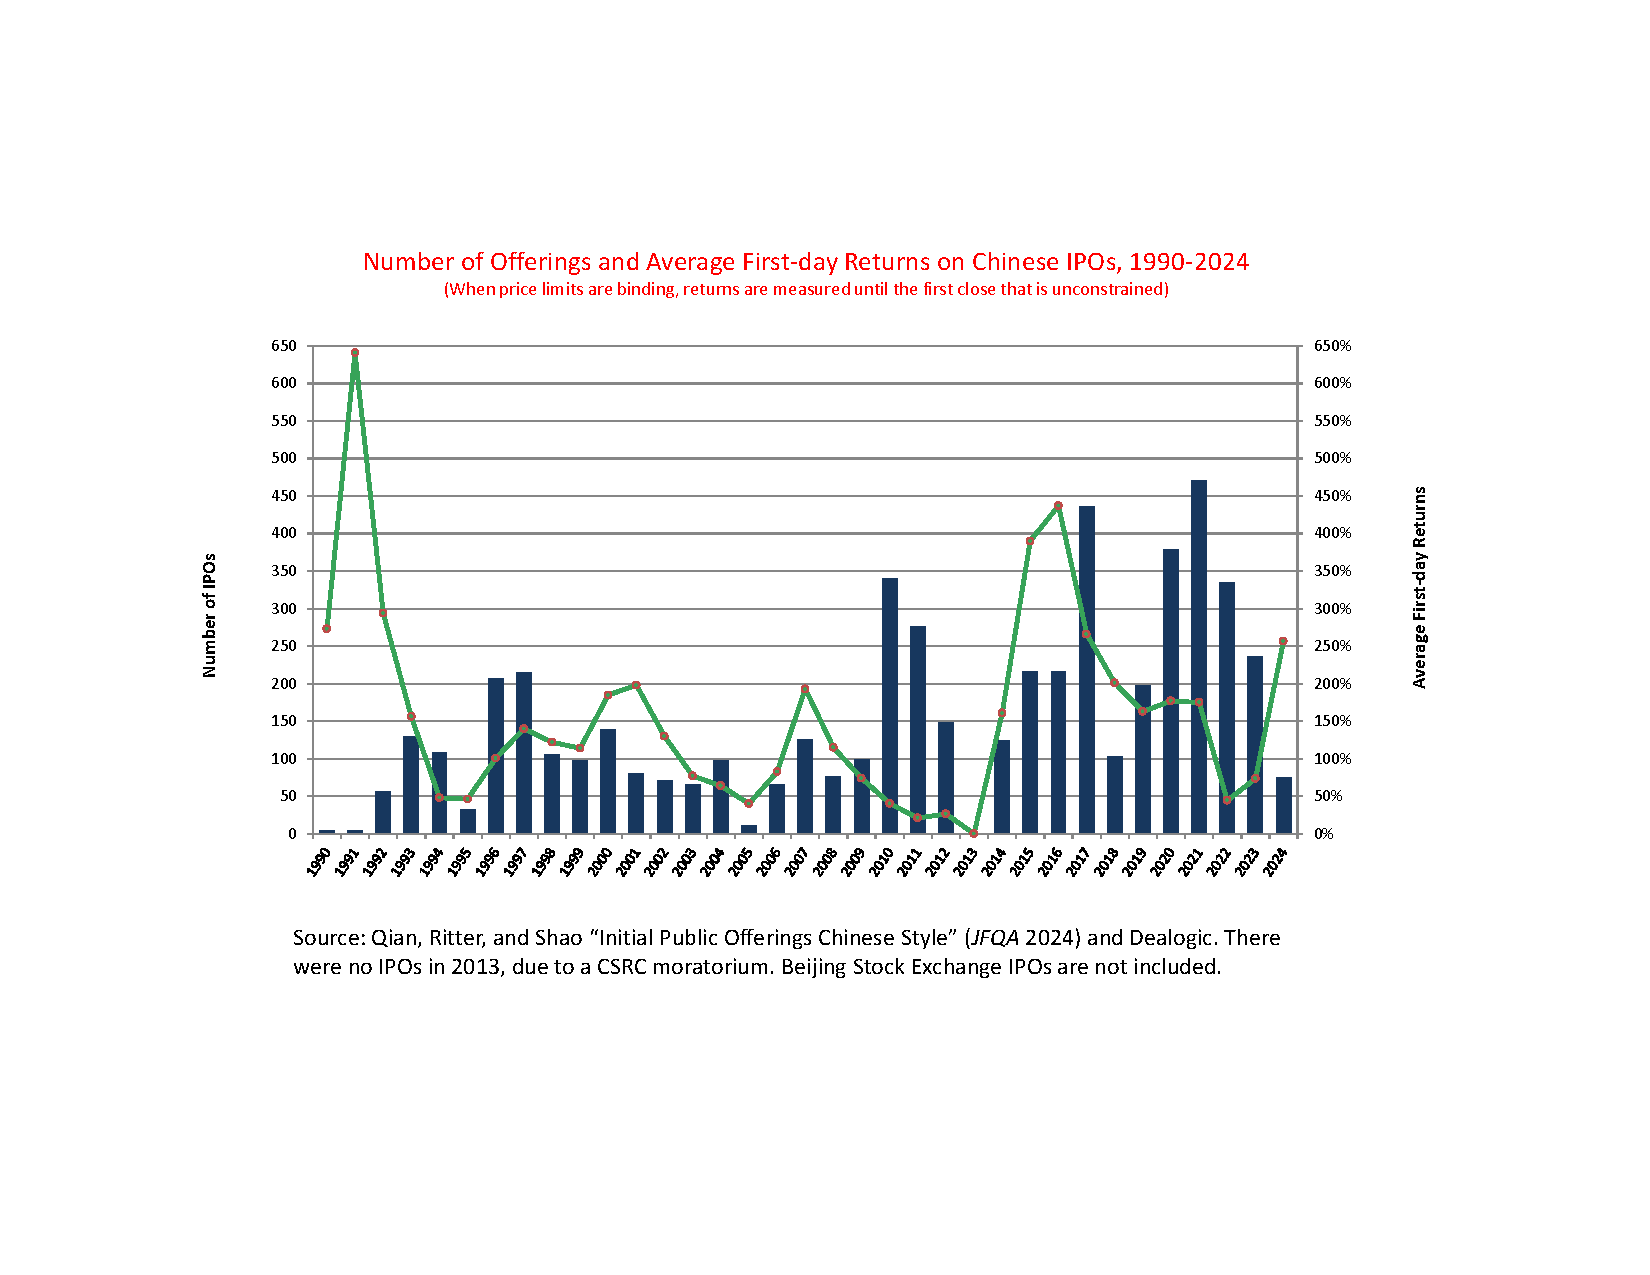
\includegraphics[width=\linewidth]{Files/IPOs-China.pdf}
\end{figure}
\end{frame}


\begin{frame}{Main Contribution}
\begin{block}{Core Idea}
Define \textbf{IPOFDR} (IPO First-Day Return) as \textit{minus} the average IPO 1st-day return:
\[
\text{IPOFDR}_t = -\frac{1}{N_t}\sum_{i=1}^{N_t} r_{i,t}
\]
where $r_{i,t}$ is the 1st-day return of IPO $i$ and $N_t$ is the number of IPOs in period $t$.
\end{block}

\textbf{Main Argument:} IPOFDR is a proxy of \textbf{ex ante equity premium}

\textbf{Three Empirical Tests:}
\begin{enumerate}
    \item Positive relation between IPOFDR and future market returns
    \item Changes in IPOFDR explain cross-section of stock returns
    \item IPOFDR correlates with market variance and idiosyncratic variance
\end{enumerate}
\end{frame}

\begin{frame}{Implications}
\begin{itemize}
    \item Challenges the view that IPO 1st-day return measures \textbf{investor sentiment} (\href{https://doi.org/10.1111/j.1540-6261.2006.00885.x}{\textcolor{blue}{Baker and Wurgler, 2006}})
    
    \item Consistent with \textbf{rational pricing} models:
    \begin{itemize}
        \item \href{https://doi.org/10.1111/j.1540-6261.2005.00778.x}{\textcolor{blue}{Pástor and Veronesi (2005)}}: Optimal IPO timing with time-varying discount rates
        \item Time-varying discount rates significantly affect IPO market valuation
    \end{itemize}
    
    \item Provides a direct measure of ex ante equity premium for empirical research

    \item Helps uncover the negative relation between dividend yield and future dividend growth (\href{https://doi.org/10.1093/rfs/1.3.195}{\textcolor{blue}{Campbell and Shiller, 1988}})
\end{itemize}
\end{frame}


\begin{frame}{Campbell-Shiller Present Value Relation}
\begin{block}{Market Price of IPO Shares (Investor's Perspective)}
Following Campbell and Shiller (1988), the log market price equals:
\[
p_{i,t} = \left(\frac{k}{1-\rho}\right)_i + E_t\left[\sum_{j=0}^{\infty}\rho^j\left((1-\rho)d_{i,t+1+j} - r_{i,t+1+j}\right)\right]
\]
\end{block}

\textbf{Notation:}
\begin{itemize}
    \item $p_{i,t}$: Log market price of IPO $i$ at time $t$
    \item $\left(\frac{k}{1-\rho}\right)_i$: Firm-specific constant
    \item $E_t$: Expectation based on \textbf{investors'} information set
    \item $d_{i,t+1+j}$: Log dividend at time $t+1+j$
    \item $r_{i,t+1+j}$: Log equilibrium discount rate
    \item $\rho$: Discount factor in linearization (typically $\approx 0.96$)
\end{itemize}
\end{frame}

\begin{frame}{Offer Price: Issuer's Perspective}
\begin{block}{Log-Linearized Offer Price}
Apply Campbell-Shiller linearization to the offer price:
\[
P_{i,t}^O = \left(\frac{k}{1-\rho}\right)_i^O + E_t^O\left[\sum_{j=0}^{\infty}\rho^j\left((1-\rho)d_{i,t+1+j} - r_{i,t+1+j}^O\right)\right]
\]
\end{block}

\textbf{Key Differences:}
\begin{itemize}
    \item $E_t^O$: Expectation based on \textbf{issuers'} information set
    \item $r_{i,t+1+j}^O$: Discount rate \textbf{adopted by issuers}
    \item The offer price is \textbf{not} directly determined by market equilibrium
    \item $r_{i,t+1+j}^O$ is an \textbf{implied discount rate} that equates offer price with expected cash flows
\end{itemize}
\end{frame}

\begin{frame}[allowframebreaks]{Decomposition of IPO 1st-Day Return}

The IPO 1st-day return is the difference between market price and offer price:
\begin{align*}
ipofdr_{i,t} &= P_{i,t} - P_{i,t}^O \\[8pt]
&= c_i + \underbrace{\left(E_t - E_t^O\right)\left[\sum_{j=0}^{\infty}\rho^j(1-\rho)d_{i,t+1+j}\right]}_{\text{Underpricing of Fundamentals}}\\[8pt]
&\quad + \underbrace{\left[E_t\left(-\sum_{j=0}^{\infty}\rho^j r_{i,t+1+j}\right) - E_t^O\left(-\sum_{j=0}^{\infty}\rho^j r_{i,t+1+j}^O\right)\right]}_{\text{Underpricing of Discount Rates}}
\end{align*}

where $c_i = \left(\frac{k}{1-\rho}\right)_i - \left(\frac{k}{1-\rho}\right)_i^O$ is a constant.
\end{frame}


\begin{frame}{Two Sources of Underpricing}
\textbf{IPO 1st-day return is positive if:}


\begin{enumerate}
    \item \textbf{Underpricing of Fundamentals:}
    \[
    \left(E_t - E_t^O\right)\left[\sum_{j=0}^{\infty}\rho^j(1-\rho)d_{i,t+1+j}\right] > 0
    \]
    Investors are more optimistic about cash flows than issuers
    
    \vspace{0.5cm}
    \item \textbf{Underpricing of Discount Rates:}
    \[
    E_t\left(-\sum_{j=0}^{\infty}\rho^j r_{i,t+1+j}\right) > E_t^O\left(-\sum_{j=0}^{\infty}\rho^j r_{i,t+1+j}^O\right)
    \]
    Investors require lower expected discount rates than issuers
\end{enumerate}
\end{frame}

\begin{frame}{Why Underpricing of Fundamentals is Unlikely}
\begin{alertblock}{Argument 1: Issuers' Incentives}
\begin{itemize}
    \item Underestimating fundamentals \textbf{lowers} the offer price (against issuers' interests)
    \item Understating cash flows in prospectus undermines investor confidence
    \item May even jeopardize the outcome of IPOs
    \item \textbf{Optimal strategy:} Adjust offer price through discount rate, not fundamentals
\end{itemize}
\end{alertblock}

\begin{alertblock}{Argument 2: Investor Rationality}
\begin{itemize}
    \item No reason for rational investors to be more optimistic than issuers
    \item Issuers have \textbf{superior information} about their own firms
    \item Issuers have incentives to \textbf{exaggerate} fundamentals
\end{itemize}
\end{alertblock}
\end{frame}

\begin{frame}{Key Assumption: Averaging Out Idiosyncratic Differences}
\begin{block}{Assumption 1: Cash Flow Expectations}
If both investors and issuers are rational, differences in cash flow expectations are \textbf{idiosyncratic}:
\[
\frac{1}{N_t}\sum_{i}^{N_t}\left(E_t - E_t^O\right)\left[\sum_{j=0}^{\infty}\rho^j(1-\rho)d_{i,t+1+j}\right] \approx 0
\]
\end{block}

\textbf{Implication:} With a large number of IPOs ($N_t$ large), the average difference in cash flow expectations is approximately zero.

\textbf{Consistent with \href{https://onlinelibrary.wiley.com/doi/10.1111/1540-6261.00478}{\textcolor{blue}{Ritter and Welch (2002)}}:} ``Simple fundamental misvaluation or asset pricing risk premia are unlikely to explain the average first-day return of 18.8\%.''
\end{frame}


\begin{frame}{The Partial Adjustment Phenomenon}
\begin{alertblock}{Empirical Evidence (\href{https://www.sciencedirect.com/science/article/pii/0304405X93900198}{\textcolor{white}{Hanley, 1993}})}
Issuers adjust the final offer price \textbf{only partially} to favorable pricing information gathered during bookbuilding.
\end{alertblock}

\textbf{Theoretical Explanations:}
\begin{itemize}
    \item \textbf{Benveniste and Spindt (1989):} Compensation to investors for revealing favorable private information
    \item \textbf{Loughran and Ritter (2002):} Agency conflicts between issuers and underwriters
    \item \textbf{Edelen and Kadlec (2005):} Trade-off between IPO proceeds and probability of success
\end{itemize}

\begin{alertblock}{Key Insight}
Partial adjustment is \textbf{crucial} for establishing the link between IPOFDR and ex ante equity premium.
\end{alertblock}
\end{frame}

\begin{frame}[allowframebreaks]{Partial Adjustment Assumption}
\begin{block}{Mathematical Formulation}
Issuers adjust their discount rates only partially to expected investors' discount rates:
\[
E_t^O\left(\sum_{j=0}^{\infty}-\rho^j r_{i,t+1+j}^O\right) = \alpha_{it}E_t^O\left(\sum_{j=0}^{\infty}-\rho^j r_{i,t+1+j}\right) - \mu_{it}
\]
\end{block}

\textbf{Parameters:}
\begin{itemize}
    \item $\alpha_{it} < 1$: Degree of adjustment (partial adjustment implies $\alpha_{it} < 1$)
    \item $\mu_{it}$: Captures effects of other explanations (e.g., asymmetric information by Rock (1986), legal considerations by Tinic (1988))
\end{itemize}

\framebreak
\begin{block}{Assumption 2: Time-Stable Non-Adjustment Component}
\[
\frac{1}{N_t}\sum_{i}^{N_t}(-\mu_{it}) \approx -\mu \quad \text{(approximately constant)}
\]
\end{block}
\end{frame}

\begin{frame}[allowframebreaks]{Deriving the Underpricing of Discount Rates}
Using the partial adjustment assumption:
\begin{align*}
&E_t\left(-\sum_{j=0}^{\infty}\rho^j r_{i,t+1+j}\right) - E_t^O\left(-\sum_{j=0}^{\infty}\rho^j r_{i,t+1+j}^O\right) \\[10pt]
&= (1-\alpha_{it})E_t\left[\sum_{j=0}^{\infty}(-\rho^j r_{i,t+1+j})\right] \\[8pt]
&\quad + \alpha_{it}\underbrace{\left(E_t - E_t^O\right)\left[\sum_{j=0}^{\infty}(-\rho^j r_{i,t+1+j})\right]}_{\text{Idiosyncratic, averages to zero}} + \mu_{it}
\end{align*}

\framebreak
\begin{block}{Assumption 3: Idiosyncratic Discount Rate Expectations}
\[
\frac{1}{N_t}\sum_{i}^{N_t}\alpha_{it}\left(E_t - E_t^O\right)\left[\sum_{j=0}^{\infty}(-\rho^j r_{i,t+1+j})\right] \approx 0
\]
\end{block}
\end{frame}

\begin{frame}[allowframebreaks]{Average IPO Underpricing}
Combining all assumptions, the average IPO 1st-day return:
\begin{block}{Key Equation}
\[
\frac{1}{N_t}\sum_{i=1}^{N_t}ipofdr_{i,t} \approx c + \mu + \frac{1}{N_t}\sum_{i=1}^{N_t}\left[(1-\alpha_{it})E_t\sum_{j=0}^{\infty}(-\rho^j r_{i,t+1+j})\right]
\]
\end{block}

\textbf{Decomposing $\alpha_{it}$:}
\[
\alpha_{it} = \alpha_t + \eta_{it}
\]
\begin{itemize}
    \item $\alpha_t$: Systematic component (varies with market conditions)
    \item $\eta_{it}$: Idiosyncratic component (averages to zero)
\end{itemize}
\framebreak
\begin{block}{Assumption 4: Idiosyncratic Adjustment Component}
\[
\frac{1}{N_t}\sum_{i=1}^{N_t}\eta_{it}E_t\sum_{j=0}^{\infty}\rho^j r_{i,t+1+j} = 0
\]
\end{block}
\end{frame}


\begin{frame}{Linking to Market Returns}
\begin{block}{Cross-Sectional Average to Market Returns}
For large $N_t$, the cross-sectional average of expected discount rates approximates expected market returns:
\[
\frac{1}{N_t}\sum_{i=1}^{N_t}\left(E_t\sum_{j=0}^{\infty}\rho^j r_{i,t+1+j}\right) \approx E_t\sum_{j=0}^{\infty}\rho^j r_{m,t+1+j}
\]
\end{block}


\textbf{Caveat:} IPO firms tend to be young, small growth firms, so their discount rates may not be fully representative of market returns.


\textbf{However:} Campbell and Vuolteenaho (2004) show that valuation of young, small growth stocks is \textbf{very sensitive} to changes in aggregate discount rates $\Rightarrow$ Strong correlation expected.
\end{frame}

\begin{frame}{Final Model: IPOFDR as Ex Ante Equity Premium}

\[
\frac{1}{N_t}\sum_{i=1}^{N_t}r_{i,t} \approx c + \mu - (1-\alpha_t)E_t\sum_{j=0}^{\infty}\rho^j r_{m,t+1+j}
\]

\[
\boxed{\text{IPOFDR}_t = -\frac{1}{N_t}\sum_{i=1}^{N_t}r_{i,t} \approx (1-\alpha_t)E_t\sum_{j=0}^{\infty}\rho^j r_{m,t+1+j} - c - \mu}
\]

\textbf{Key Result:} Since $0 < \alpha_t < 1$ (partial adjustment), IPOFDR is \textbf{positively related} to expected future market returns!
\end{frame}

\begin{frame}{Hot vs. Cold Markets}
\begin{block}{Time-Varying Adjustment Coefficient}
\begin{itemize}
    \item $\alpha_t$ is \textbf{smaller} in hot markets (less complete adjustment)
    \item $\alpha_t$ is \textbf{larger} in cold markets (more complete adjustment)
\end{itemize}
\end{block}


\textbf{Implication:} The coefficient $(1-\alpha_t)$ is larger in hot markets:
\[
\text{IPOFDR}_t \approx \underbrace{(1-\alpha_t)}_{\text{larger in hot markets}}E_t\sum_{j=0}^{\infty}\rho^j r_{m,t+1+j} - c - \mu
\]


\begin{alertblock}{Testable Prediction}
The relation between IPOFDR and future market returns should be \textbf{stronger in hot markets} than in cold markets.
\end{alertblock}
\end{frame}


\begin{frame}{Three Testable Implications}
\begin{block}{Implication 1: Time-Series Predictability}
IPOFDR forecasts excess stock market returns:
\[
\text{ERET}_{t+1} = \theta + \gamma \cdot \text{IPOFDR}_t + \varepsilon_{t+1}
\]
\begin{itemize}
    \item $\gamma > 0$ (positive relation)
    \item $\gamma$ larger for hot markets than cold markets
\end{itemize}
\end{block}


\begin{block}{Implication 2: Cross-Sectional Pricing}
Merton's (1973) and Campbell's (1993) ICAPMs imply:
\begin{itemize}
    \item Innovations in IPOFDR ($\Delta$IPOFDR) are a \textbf{priced risk factor}
    \item Should help explain cross-section of stock returns
\end{itemize}
\end{block}
\end{frame}

\begin{frame}{Testable Implications (Continued)}
\begin{block}{Implication 3: Correlation with Systematic Risk}
IPOFDR should correlate with measures of systematic risk:
\begin{itemize}
    \item \textbf{Market Variance (MV):} Positive correlation
    \item \textbf{Average Idiosyncratic Variance (IV):} Negative correlation
\end{itemize}
\end{block}


\textbf{ICAPM Framework (Guo and Savickas, 2008):}
\begin{itemize}
    \item Conditional equity premium depends on:
    \begin{itemize}
        \item Conditional variance of market returns (MV)
        \item Conditional variance of hedging factor (proxied by IV)
    \end{itemize}
    \item MV positively related to future returns
    \item IV negatively related to future returns (hedging demand)
\end{itemize}
\end{frame}


\begin{frame}{Data and Sample}
\textbf{Data Sources:}
\begin{itemize}
    \item Monthly IPO 1st-day returns and number of IPOs: Jay Ritter (U. of Florida)
    \item Sample period: January 1960 -- December 2006
    \item Market returns: S\&P 500 value-weighted index
    \item Fama-French factors: Kenneth French (Dartmouth)
\end{itemize}

\textbf{Annual Data Used Because:}
\begin{enumerate}
    \item Missing observations at monthly/quarterly frequency (e.g., July--Dec 1974)
    \item Larger sample of IPOs per period provides reliable measure
    \item IPOFDR may forecast better at longer horizons
\end{enumerate}
\end{frame}

\begin{frame}{Result : Forecasting Market Returns}
\begin{block}{Forecasting Regression}
\[
\text{ERET}_{t+1} = \theta + \gamma \cdot \text{IPOFDR}_t + \eta_{t+1}
\]
\end{block}

\begin{table}[h]
\centering
\small
\begin{tabular}{lccc}
\toprule
Period & IPOFDR Coefficient & $R^2$ \\
\midrule
1961--2006 & $0.392^{**}$ & 0.108 \\
1961--1982 & $0.317$ & 0.038 \\
1983--2006 & $0.501^{**}$ & 0.187 \\
1961--1995 & $0.355$ & 0.051 \\
\bottomrule
\end{tabular}
\end{table}

\textbf{Key Finding:} IPOFDR significantly predicts future excess market returns with $R^2 \approx 11\%$ in full sample.
\end{frame}

\begin{frame}{Hot vs. Cold Market Effects}
\begin{block}{Extended Model with Dummy Variable}
\[
\text{ERET}_{t+1} = \theta + \gamma \cdot \text{IPOFDR}_t + \delta \cdot \text{IPOFDR}_t \times \text{DUM}_t + \eta_{t+1}
\]
where DUM = 1 if number of IPOs $< 200$ (cold market), 0 otherwise.
\end{block}

\begin{table}[h]
\centering
\small
\begin{tabular}{lcccc}
\toprule
Period & IPOFDR & IPOFDR $\times$ DUM & $\gamma + \delta$ & $R^2$ \\
\midrule
1961--2006 & $0.407^{**}$ & $-0.177$ & 0.230 & 0.096 \\
1961--1982 & $0.412^{*}$ & $-0.403^{*}$ & 0.009 & 0.053 \\
1983--2006 & $0.524^{**}$ & $0.327$ & 0.850 & 0.160 \\
\bottomrule
\end{tabular}
\end{table}

\textbf{Interpretation:} Predictive power stronger in hot markets ($\gamma$) than cold markets ($\gamma + \delta$), consistent with theory.
\end{frame}


\begin{frame}{Machine Learning in Return Prediction}
	\textbf{Recent advances}:
	\begin{itemize}
		\item \href{https://doi.org/10.1093/rfs/hhaa009}{\textcolor{blue}{Gu, Kelly, and Xiu (2020)}}: Comprehensive ML comparison
		\begin{itemize}
			\item Neural networks, random forests, gradient boosting
			\item Significant out-of-sample $R^2$ improvements
		\end{itemize}
		\item \href{https://doi.org/10.1016/j.jfineco.2020.06.017}{\textcolor{blue}{Rapach, Strauss, Tu, and Zhou (2019)}}: LASSO and Ridge for forecasting
		\item \href{https://doi.org/10.1093/rfs/hhab086}{\textcolor{blue}{Cong, Tang, Wang, and Zhang (2021)}}: Deep learning for China's market
		\item \href{https://doi.org/10.1093/rfs/hhab123}{\textcolor{blue}{Gu, Kelly, and Xiu (2021)}}: Autoencoder asset pricing models
	\end{itemize}
	
	\vspace{5pt}
	\textbf{Key finding}: Combining multiple predictors via ML often outperforms individual predictors.
\end{frame}

\begin{frame}{Combination Forecasts}
	\href{https://doi.org/10.1093/rfs/hhq033}{\textcolor{blue}{Rapach, Strauss, and Zhou (2010)}}: Forecast combinations
	
	\vspace{5pt}
	\textbf{Simple average}:
	\begin{align*}
		\hat{r}_{t+1}^{comb} = \frac{1}{N}\sum_{i=1}^{N}\hat{r}_{t+1}^{(i)}
	\end{align*}
	
	\textbf{Key findings}:
	\begin{itemize}
		\item Simple average often beats individual forecasts
		\item Reduces model uncertainty and estimation error
		\item Robust to structural breaks
	\end{itemize}
	
	\vspace{5pt}
	\href{https://doi.org/10.1016/j.jfineco.2017.05.012}{\textcolor{blue}{Huang, Jiang, Tu, and Zhou (2017)}}: LASSO-based combination with constraints
\end{frame}

\begin{frame}{Recent Literature: 2020-2025}
	\textbf{Methodological advances}:
	\begin{itemize}
		\item \href{https://doi.org/10.1093/rfs/hhae044}{\textcolor{blue}{Goyal, Welch, and Zafirov (2024)}}: Comprehensive update
		\begin{itemize}
			\item More than one-third of new variables lose in-sample significance
			\item Half of remaining have poor out-of-sample performance
		\end{itemize}
		\item \href{https://doi.org/10.1093/rfs/hhaf010}{\textcolor{blue}{Li, Rossi, and Zhou (2025)}}: Hybrid forecasting framework
		\begin{itemize}
			\item Combines bias-reduction with historical average
			\item Outperforms conventional methods across economic cycles
		\end{itemize}
	\end{itemize}
\end{frame}

\subsection{\href{https://doi.org/10.1093/rfs/hhaf010}{\textcolor{blue}{Li, Rossi, and Zhou (2025)}}}

\begin{frame}{\href{https://doi.org/10.1093/rfs/hhaf010}{\textcolor{blue}{Li, Rossi, and Zhou (2025)}}: The Challenge of Equity Premium Prediction}
	\textbf{The Gold Standard: Historical Average}
	\begin{itemize}
		\item The historical average is the current benchmark for forecasting equity premium
		\item Goyal and Welch (2008): Many predictors perform poorly in \textbf{out-of-sample (OOS)} forecasts
		\item Goyal, Welch, and Zafirov (2024): Confirm these findings over longer periods
	\end{itemize}
	
	\textbf{Campbell and Thompson (2008) posed the question:} ``Can anything beat the historical average?''
	\textbf{This paper's answer:} \textcolor{blue}{Yes, by targeting a lower bias rather than unbiasedness!}
\end{frame}

\begin{frame}{Main Contribution}
	\textbf{A Novel Methodology for OOS Forecasting}
	
	
	\textbf{Key Innovation:}
	\begin{itemize}
		\item Use a \textbf{conservative constant} as the predictive slope coefficient
		\item This constant has:
		\begin{itemize}
			\item \textbf{Lower bias} than the zero slope of historical average
			\item \textbf{Same variance} (zero) as the historical average
		\end{itemize}
	\end{itemize}
	
	
	\textbf{Theoretical Results:}
	\begin{itemize}
		\item The proposed forecast \textbf{first-order stochastically dominates} the historical average
		\item Lower mean squared forecast error when population slope $\neq 0$
	\end{itemize}
	
	
	\textbf{Empirical Results:}
	\begin{itemize}
		\item 15 of 23 predictors achieve significant positive OOS $R^2$ at 90\% level
		\item 8 predictors significant at 95\% level
	\end{itemize}
\end{frame}

\begin{frame}{Intuition: The ``Price Is Right'' Game}
	\textbf{A Guess-the-Number Game Analogy}
	
	\vspace{0.2cm}
	\begin{itemize}
		\item Competitors guess the actual slope coefficient $b$ of a predictor
		\item \textbf{Mr. Historical Average} guesses \textbf{zero}
		\item Suppose the true slope is $b = 1$
	\end{itemize}
	
	
	\textbf{OLS Approach (estimation variance = 1):}
	\begin{itemize}
		\item Loses to Mr. Historical Average if estimate is $<0$ or $>2$
		\item High variance makes OLS unreliable
	\end{itemize}
	
	
	\textbf{The Authors' Approach:}
	\begin{itemize}
		\item Guess a \textbf{conservative positive constant}, e.g., $\delta = 0.2$
		\item Beats Mr. Historical Average unless true $b < 0.1$
		\item \textcolor{blue}{Conservative + deterministic = bias reduction with zero variance}
	\end{itemize}
\end{frame}


\begin{frame}{Model Setup}
	\textbf{Predictive Regression:}
	\begin{equation}
		r = \mu + bx + e
	\end{equation}
	
	where:
	\begin{itemize}
		\item $r$: future return
		\item $x$: predictor (zero mean)
		\item $b$: predictive slope coefficient
		\item $e$: residual (zero mean, uncorrelated with $x$)
		\item $\mu$: unconditional expected return
	\end{itemize}
	
	
	\textbf{Historical Average Estimation:}
	\begin{equation}
		\mu = \hat{\mu} + \xi
	\end{equation}
	where $\hat{\mu}$ is the historical average and $\xi$ has zero mean.
	
	\vspace{0.2cm}
	\textbf{Combined Form:}
	\begin{equation}
		r = \hat{\mu} + bx + \epsilon, \quad \text{where } \epsilon \equiv e + \xi
	\end{equation}
\end{frame}

\begin{frame}{Theorem 1: First-Order Stochastic Dominance (Population Mean)}
	\textbf{Theorem 1:} The forecast $\mu + \delta x$ \textbf{first-order stochastically dominates} the forecast $\mu$ under:
	
	
	\textbf{Conditions:}
	\begin{enumerate}
		\item $\delta$ is a constant between 0 and $b$
		\item The PDF of vector $\mathbf{e}$ is strictly decreasing in $\|\mathbf{e}\|$
	\end{enumerate}
	
	
	\textbf{Definition of First-Order Stochastic Dominance:}
	\begin{itemize}
		\item $A$ dominates $B$ if: $P(A \geq c) \geq P(B \geq c)$ for all $c$
		\item And $P(A \geq c) > P(B \geq c)$ for some $c$
	\end{itemize}
	
	
	\textbf{Implication:} Anyone with strictly increasing utility over gains prefers forecast A to B (Huang and Litzenberger, 1988)
\end{frame}

\begin{frame}{Theorem 2: First-Order Stochastic Dominance (Estimated Mean)}
	\textbf{Theorem 2:} The forecast $\hat{\mu} + \delta x$ \textbf{first-order stochastically dominates} the forecast $\hat{\mu}$ (historical average) under:
	
	
	\textbf{Conditions:}
	\begin{enumerate}
		\item $\delta$ is a constant between 0 and $b$
		\item The PDF of vector $\boldsymbol{\epsilon}$ is strictly decreasing in $\|\boldsymbol{\epsilon}\|$
	\end{enumerate}
	
	
	\textbf{Corollary 1:}
	\begin{equation}
		\text{MSE}_{\hat{\mu}+\delta x} \overset{d}{=} \text{MSE}_{\hat{\mu}} - \eta, \quad \eta \geq 0
	\end{equation}
	
	\vspace{0.2cm}
	\textbf{Key Insight:}
	\begin{itemize}
		\item Monotonicity restriction holds for $t$-distribution and normal distribution
		\item Zero variance matching + bias reduction $\Rightarrow$ lower MSE
	\end{itemize}
\end{frame}

\begin{frame}{Implementation: Predictive Slope Selection}
	\textbf{Predictive Slope:}
	\begin{equation}
		\delta = \begin{cases}
			1/A & \text{if } b > 0 \\
			-1/A & \text{if } b < 0
		\end{cases}
	\end{equation}
	where $A > 0$ is a constant.
	
	
	\textbf{Larger $A$:}
	\begin{itemize}
		\item Ensures $\delta$ is between 0 and $b$ (required by Theorem 2)
		\item More conservative (smaller magnitude)
	\end{itemize}
	
	
	\textbf{Sign Determination:}
	\begin{enumerate}
		\item \textbf{Economic theory}: Campbell and Thompson (2008) restrictions
		\item \textbf{Statistical inference}: Confidence intervals
		\item \textbf{Previous studies}: Published estimates
	\end{enumerate}
\end{frame}

\begin{frame}{Using Confidence Intervals}
	\textbf{For Significantly Positive Slope:}
	
	Consider 95\% confidence interval $[\hat{b}_L, \hat{b}_U]$:
	\begin{equation}
		0 < \hat{b}_L \leq b \leq \hat{b}_U \quad \text{(with 95\% probability)}
	\end{equation}
	
	\vspace{0.2cm}
	\textbf{Setting $\delta$ to lower confidence bound:}
	\begin{itemize}
		\item $\delta = 1/A = \hat{b}_L$ ensures $\delta$ between 0 and $b$ with high probability
	\end{itemize}
	
	
	\textbf{Example: Campbell and Shiller (1988a)}
	\begin{itemize}
		\item Dividend-price ratio: slope = 0.129, SE = 0.057, $\sigma_x = 0.277$
		\item 95\% lower bound for standardized predictor:
		\begin{equation}
			(0.129 - 1.96 \times 0.057) \times 0.277 = 0.0048
		\end{equation}
		\item This implies $A = 1/0.0048 = 209$
	\end{itemize}
\end{frame}

\begin{frame}{Theorems 3 \& 4: Uncertainty About Sign}
	\textbf{When Sign is Inferred with Error:}
	\begin{equation}
		d = \begin{cases}
			\delta & \text{with probability } p \text{ (correct sign)} \\
			-\delta & \text{with probability } q \text{ (wrong sign)} \\
			0 & \text{with probability } 1-p-q \text{ (undetermined)}
		\end{cases}
	\end{equation}
	
	
	\textbf{Theorem 3 \& 4:} First-order stochastic dominance holds when:
	\begin{equation}
		\frac{p}{q} > \max(B_1, B_2)
	\end{equation}
	
	\vspace{0.2cm}
	\textbf{Lemma 1 (Student's $t$ distribution):}
	\begin{equation}
		B_1 > \frac{2b + \delta}{2b - \delta}
	\end{equation}
	
	\textbf{Rule of Thumb:}
	\begin{itemize}
		\item When $\delta/b \approx 0$: $\frac{2b+\delta}{2b-\delta} \approx 1$, any $p/q > 1$ suffices
		\item At maximum $\delta/b = 1$: requires $p/q > 3$
		\item 95\% significance: $p/q \geq 0.95/0.05 = 19 \gg 3$ \checkmark
	\end{itemize}
\end{frame}


\begin{frame}{Why is the Historical Average Hard to Beat?}
	\textbf{OOS MSE Difference:}
	\begin{align}
		E\left[\text{MSE}_{\hat{\mu}} - \text{MSE}_{\hat{\mu}+\hat{b}x}\right] &= \left(b^2 - \text{Bias}(\hat{b})^2 - \text{Var}(\hat{b})\right)x^2 \notag \\
		&\quad - 2E\left[(\hat{\mu}-\mu)\hat{b}\right]x
	\end{align}
	
	
	\textbf{Historical Average's Advantage:}
	\begin{itemize}
		\item Zero slope $\Rightarrow$ zero estimation variance
		\item High variance of $\hat{b}$ can offset bias reduction
	\end{itemize}
	
	
	\textbf{Our Method's Solution:}
	\begin{itemize}
		\item Use \textbf{constant} slope $\delta$ $\Rightarrow$ zero variance (like historical average)
		\item Last term becomes zero when $\hat{b}$ is constant and $\hat{\mu}$ unbiased
		\item MSE difference $= (b^2 - \text{Bias}(\delta)^2)x^2 > 0$ when $\delta$ between 0 and $b$
	\end{itemize}
\end{frame}

\begin{frame}{Gradient Descent Interpretation}
	\textbf{Gradient Descent:}
	\begin{equation}
		a_1 = a_0 - \gamma f'(a_0)
	\end{equation}
	
	\vspace{0.2cm}
	\textbf{Mapping to Our Method:}
	\begin{itemize}
		\item $f$: forecast loss function
		\item $a$: predictive slope
		\item Historical average: initial guess $a_0 = 0$
		\item Our method: $a_1 = \delta = 1/A$
	\end{itemize}
	
	
	\textbf{Interpretation:}
	\begin{itemize}
		\item Our predictive slope = one step from zero toward predictability
		\item Step direction: guided by sign of population slope $b$
		\item Step size: constant $1/A$ (matches zero variance)
	\end{itemize}
\end{frame}

\begin{frame}{Amortization Interpretation}
	\textbf{Standardized Predictor (e.g., $dp$):}
	\begin{itemize}
		\item $dp = 0$: at mean, no effect on forecast
		\item $dp = -1$: one standard deviation below mean (price excessively high)
	\end{itemize}
	
	
	\textbf{Amortization of Excess Valuation:}
	\begin{itemize}
		\item Slope $1/A$ $\approx$ mean reversion rate
		\item Example: $A = 100$ $\Rightarrow$ 1\% mean reversion per period
	\end{itemize}
	
	
	\textbf{Connection to AR(1) Process:}
	\begin{itemize}
		\item If $dp$ follows AR(1) with coefficient $\rho$
		\item Linear approximation: mean reversion rate $\approx 1 - \rho$
		\item Setting $1/A = 1 - \rho$ matches the dynamics
		\item Persistent predictors ($\rho \approx 1$) $\Rightarrow$ large $A$
	\end{itemize}
\end{frame}

\begin{frame}{Better Limit for Shrinkage}
	\textbf{Traditional Shrinkage:}
	\begin{itemize}
		\item Shrink regression estimate toward a constant limit (often zero)
		\item Still produces a \textbf{random} estimator
	\end{itemize}
	
	
	\textbf{Our Approach:}
	\begin{itemize}
		\item Slope $\delta$ is \textbf{constant} (not random)
		\item Matches zero variance while reducing bias
		\item Enables \textbf{ex ante} characterization of superior performance
	\end{itemize}
	
	
	\textbf{Improvement to Shrinkage:}
	\begin{itemize}
		\item Historical average (zero) is biased when predictability exists
		\item Bias can be same magnitude as estimation standard deviation
		\item Replace zero limit with our forecast for better shrinkage performance
	\end{itemize}
\end{frame}


\begin{frame}{Simulation Setup}
	\textbf{VAR System (Cochrane, 2008):}
	\begin{align}
		r_{t+1} &= a_r + b_r \cdot dp_t + \varepsilon^r_{t+1} \\
		dp_{t+1} - \overline{dp} &= \rho(dp_t - \overline{dp}) + \varepsilon^{dp}_{t+1} \\
		\Delta d_{t+1} &= a_d + b_d \cdot dp_t + \varepsilon^d_{t+1}
	\end{align}
	
	\vspace{0.2cm}
	\textbf{Calibration Parameters:}
	\begin{center}
		\begin{tabular}{lc}
			\toprule
			Parameter & Value \\
			\midrule
			$\overline{dp}$ & $-3.2239$ \\
			$\rho$ & $0.8911$ \\
			$\kappa_1$ & $0.9617$ \\
			$b_d$ & $0$ \\
			$b_r = 1 - \kappa_1\rho + b_d$ & $0.1430$ \\
			\bottomrule
		\end{tabular}
	\end{center}
	
	\vspace{0.2cm}
	Rolling 20-year windows for estimation
\end{frame}

\begin{frame}{Bias-Variance Trade-off}
	\begin{columns}
		\begin{column}{0.5\textwidth}
			\textbf{Bias of Predictive Slope:}
			\begin{itemize}
				\item HM: biased (uses zero slope)
				\item Our method ($A=50$): smaller bias
				\item OLS: Stambaugh (1999) bias
			\end{itemize}
			
			
			\textbf{Standard Deviation:}
			\begin{itemize}
				\item HM: zero
				\item Our method: \textbf{zero}
				\item OLS: large (almost equals HM bias!)
			\end{itemize}
		\end{column}
		\begin{column}{0.5\textwidth}
			\textbf{RMSE of Slope:}
			\begin{itemize}
				\item Our method has \textbf{smallest RMSE}
				\item Same zero variance as HM
				\item But smaller bias than HM
			\end{itemize}
			
			
			\textbf{Key Insight:}
			\begin{itemize}
				\item OLS variance $\approx$ HM bias
				\item Variance can offset bias reduction
				\item Our method: pure bias reduction
			\end{itemize}
		\end{column}
	\end{columns}
\end{frame}

\begin{frame}{OOS $R^2$ Distribution}
	\textbf{OOS $R^2$ Definition:}
	\begin{equation}
		R^2 = \frac{\text{MSE}_{\hat{\mu}} - \text{MSE}_{\hat{\mu}+\delta x}}{\text{MSE}_{\hat{\mu}}}
	\end{equation}
	
	
	\textbf{Simulation Results (146 annual returns):}
	\begin{itemize}
		\item \textbf{Our method} ($A = 50$ to 500):
		\begin{itemize}
			\item Distributions entirely to the \textbf{right of zero}
			\item Confirms Corollary 1: lower MSE than HM
			\item Larger $A$ $\Rightarrow$ smaller but less noisy gains
		\end{itemize}
		
		\vspace{0.2cm}
		\item \textbf{OLS}:
		\begin{itemize}
			\item Centered on positive $R^2$
			\item \textbf{Large fluctuation} (fat tails)
			\item Substantial probability of $R^2 < 0$
		\end{itemize}
	\end{itemize}
\end{frame}

\begin{frame}{First-Order Stochastic Dominance in Simulations}
	\textbf{CDF of MSE:}
	\begin{itemize}
		\item Our method's CDF is \textbf{everywhere above} HM's CDF
		\item Confirms Theorem 2
	\end{itemize}
	
	
	\textbf{Horizon Effects:}
	\begin{itemize}
		\item \textbf{1-year window:} MSE more spread out, CDFs closer together
		\item \textbf{10-year window:} Clearer separation
		\item \textbf{40-year window:} Much narrower MSE range, dominance easier to discern
	\end{itemize}
	
	
	\textbf{Implication:}
	\begin{itemize}
		\item First-order stochastic dominance holds at all horizons
		\item Longer horizons facilitate empirical inference
		\item Long-term investors benefit most clearly
	\end{itemize}
\end{frame}


\begin{frame}{Data and Predictors}
	\textbf{Data Sources:}
	\begin{itemize}
		\item Market returns: CRSP value-weighted index (post-1926), S\&P Index (pre-1926)
		\item Predictors: Goyal and Welch (2008) + Robert Shiller's website
	\end{itemize}
	
	
	\textbf{23 Predictors Examined:}
	\begin{columns}
		\begin{column}{0.5\textwidth}
			\footnotesize
			\begin{itemize}
				\item Book-to-market (bm)
				\item CAPE (cape Shiller)
				\item Consumption-wealth ratio (cay)
				\item Corporate bond return (corpr)
				\item Dividend-payout ratio (de)
				\item Dividend-price ratio (dp)
				\item Dividend yield (dy)
				\item Earnings-price ratio (ep)
			\end{itemize}
		\end{column}
		\begin{column}{0.5\textwidth}
			\footnotesize
			\begin{itemize}
				\item Investment-capital ratio (ik)
				\item Inflation (infl)
				\item Long-term return (ltr)
				\item Long-term yield (lty)
				\item Net equity issuance (ntis)
				\item Stock variance (svar)
				\item T-bill rate (tbl)
				\item Term spread (tms)
			\end{itemize}
		\end{column}
	\end{columns}
	
	\vspace{0.2cm}
	\textbf{Standardization:} 20-year rolling windows for mean and std
\end{frame}

\begin{frame}{Cumulative Performance: Dividend-Price Ratio}
	\textbf{Cumulative SSE Difference (HM minus forecast):}
	
	\vspace{0.2cm}
	\textbf{OLS Performance:}
	\begin{itemize}
		\item Volatile, driven by 1970s Oil Shock
		\item Key concern in Goyal and Welch (2008)
	\end{itemize}
	
	\vspace{0.2cm}
	\textbf{Our Method's Performance:}
	\begin{itemize}
		\item \textbf{Steady accumulation} of gains over time
		\item Works for various $A$ values (50 to 1,000)
		\item Even $A = 1,000$ (0.1\% per std dev) beats OLS at sample end
	\end{itemize}
	
	\vspace{0.2cm}
	\textbf{Dot-Com Period:}
	\begin{itemize}
		\item Biggest forecast error (high returns despite low $dp$)
		\item Loss mitigated with larger $A$ (e.g., $A \geq 200$)
		\item $A = 500$ or 1,000: minimal impact from extreme periods
	\end{itemize}
\end{frame}

\begin{frame}{OOS $R^2$ Results: Dividend-Price Ratio}
	\begin{center}
		\begin{tabular}{lccccc}
			\toprule
			& $A=1000$ & $A=500$ & $A=200$ & $A=100$ & $A=50$ \\
			\midrule
			$R^2$ (\%) & 0.2 & 0.5 & 1.1 & 2.1 & 3.4 \\
			$p$-value & (.008) & (.009) & (.012) & (.019) & (.044) \\
			\bottomrule
		\end{tabular}
	\end{center}
	
	
	\textbf{Comparison with OLS and CT Methods:}
	\begin{center}
		\begin{tabular}{lccc}
			\toprule
			& OLS & CT+ & CT++ \\
			\midrule
			$R^2$ (\%) & 0.2 & 1.3 & 1.8 \\
			$p$-value & (.477) & (.357) & (.286) \\
			\bottomrule
		\end{tabular}
	\end{center}
	
	\vspace{0.2cm}
	\textbf{Key Finding:} Our method achieves \textbf{more significant} $p$-values than all alternatives!
\end{frame}

\begin{frame}{Economic Magnitude of Gains}
	\textbf{How to Judge $R^2$ Magnitude?}
	
	Compare to squared Sharpe ratio (Campbell and Thompson, 2008):
	\begin{itemize}
		\item Annual market Sharpe ratio: 0.278
		\item Squared Sharpe ratio: $0.278^2 = 0.078$
	\end{itemize}
	
	
	\textbf{Example with $A = 100$:}
	\begin{itemize}
		\item $R^2 = 2.1\%$
		\item Proportional expected return increase: $\frac{0.021}{0.078} = \mathbf{27\%}$
	\end{itemize}
	
	
	\textbf{Interpretation:}
	\begin{itemize}
		\item An investor recognizing predictability gains 27\% higher expected return
		\item Despite ``modest'' aim of bias reduction (not unbiasedness)
		\item Nontrivial economic gains
	\end{itemize}
\end{frame}

\begin{frame}{Comprehensive Results: All Predictors}
	\textbf{95\% Significant OOS $R^2$ (8 predictors):}
	\begin{itemize}
		\item CAPE, Total Return CAPE (Campbell and Shiller, 1988b; Bunn and Shiller, 2014)
		\item Dividend-price ratio, Dividend yield
		\item Consumption-wealth ratio (Lettau and Ludvigson, 2001)
		\item Investment-capital ratio (Cochrane, 1991)
		\item Long-term rate of returns
		\item Corporate bond returns
	\end{itemize}
	
	
	\textbf{90\% Significant OOS $R^2$ (7 additional predictors):}
	\begin{itemize}
		\item Book-to-market ratio
		\item Long-term government bond yield
		\item Treasury-bill rate, Term spread
		\item Inflation (Shiller data)
		\item Earnings-to-price ratio
	\end{itemize}
\end{frame}

\begin{frame}{First-Order Stochastic Dominance: Empirical Evidence}
	\textbf{Using 40-Year Rolling Windows:}
	\begin{itemize}
		\item Empirical CDF of our method \textbf{everywhere above} HM's CDF
		\item For any MSE threshold: higher probability of achieving lower MSE
	\end{itemize}
	
	
	\textbf{Confirmation:}
	\begin{itemize}
		\item Uses empirical distribution function (actual occurrences)
		\item Also confirmed with kernel smoothing
	\end{itemize}
	
	
	\textbf{Implication for Long-Term Investors:}
	\begin{itemize}
		\item First-order stochastic dominance holds empirically
		\item Any risk-averse investor prefers our forecast to HM
	\end{itemize}
\end{frame}

\begin{frame}{Using Estimates from Previous Studies}
	\textbf{Campbell and Shiller (1988a) Example:}
	\begin{itemize}
		\item Sample: 1871-1986
		\item Significantly positive slope for $dp$
		\item 95\% lower bound implies $A = 209$
	\end{itemize}
	
	
	\textbf{OOS Performance (post-1987):}
	\begin{itemize}
		\item Using positive slope with various $A$ values: positive OOS $R^2$
		\item Using $A = 209$ (95\% lower bound): positive OOS $R^2$
		\item \textbf{Published estimates add value to subsequent forecasts!}
	\end{itemize}
	
	
	\textbf{Direct Evidence of OOS Predictability:}
	\begin{itemize}
		\item Confidence bounds from prior studies help future forecasts
		\item Not data mining: uses pre-existing published numbers
		\item Similar results for Cochrane (1991) investment-capital ratio
	\end{itemize}
\end{frame}



\begin{frame}{Main Contributions}
	\textbf{1. Novel OOS Forecast Methodology}
	\begin{itemize}
		\item First method \textbf{proven ex ante} to outperform historical average
		\item Crucial for classroom teaching and practical implementation
	\end{itemize}

	\textbf{2. Theoretical Foundation}
	\begin{itemize}
		\item First-order stochastic dominance (Theorems 1-4)
		\item Characterization of required sign accuracy
	\end{itemize}
	
	\textbf{3. Implementation Guidance}
	\begin{itemize}
		\item Confidence bound near zero as nearly necessary and sufficient condition
		\item Connection to published estimates
	\end{itemize}

	\textbf{4. Strong Empirical Evidence}
	\begin{itemize}
		\item 15/23 predictors significant at 90\%, 8/23 at 95\%
		\item Solves instability concern of Goyal and Welch (2008)
	\end{itemize}
\end{frame}


\begin{frame}{Open Questions in Predictability Research}
	\begin{enumerate}
		\item \textbf{Economic vs. Statistical significance}: Even with $R^2_{OOS} > 0$, are returns economically exploitable after transaction costs?
		\item \textbf{Source of predictability}: Risk premium variation or mispricing?
		\item \textbf{Instability}: Why do predictors work in some periods but not others?
		\item \textbf{International evidence}: Do U.S. findings generalize globally?
		\item \textbf{Real-time availability}: Are predictors available to investors in real time?
	\end{enumerate}
	
	\vspace{5pt}
	\href{https://doi.org/10.1111/jofi.12612}{\textcolor{blue}{Kozak, Nagel and Santosh (2018)}}: 
	\begin{itemize}
		\item \alert{Can we distinguish between investor sentiment and risk?}  
	\end{itemize}
\end{frame}

\section{Homework}
\begin{frame}{Homework}
	\href{https://chenghang.notion.site/Homework-1-efe9cdfdfc0d439ebc7883b40680ce69?pvs=4}{\textcolor{blue}{Homework}}
\end{frame}

\end{document}
